%%%%%%%%%%%%%%%%%%%%%%%%%%%%%%%%%%%%%%%%%
% Beamer Presentation
% LaTeX Template
% Version 1.0 (10/11/12)
%
% This template has been downloaded from:
% http://www.LaTeXTemplates.com
%
% License:
% CC BY-NC-SA 3.0 (http://creativecommons.org/licenses/by-nc-sa/3.0/)
%
%%%%%%%%%%%%%%%%%%%%%%%%%%%%%%%%%%%%%%%%%

%----------------------------------------------------------------------------------------
%	PACKAGES AND THEMES
%----------------------------------------------------------------------------------------

\documentclass{beamer}

\mode<presentation> {

% The Beamer class comes with a number of default slide themes
% which change the colors and layouts of slides. Below this is a list
% of all the themes, uncomment each in turn to see what they look like.

%\usetheme{default}
%\usetheme{AnnArbor}
%\usetheme{Antibes}
%\usetheme{Bergen}
%\usetheme{Berkeley}
%\usetheme{Berlin}
%\usetheme{Boadilla}
%\usetheme{CambridgeUS}
%\usetheme{Copenhagen}
%\usetheme{Darmstadt}
%\usetheme{Dresden}
%\usetheme{Frankfurt}
%\usetheme{Goettingen}
%\usetheme{Hannover}
%\usetheme{Ilmenau}
%\usetheme{JuanLesPins}
%\usetheme{Luebeck}
\usetheme{Madrid}
%\usetheme{Malmoe}
%\usetheme{Marburg}
%\usetheme{Montpellier}
%\usetheme{PaloAlto}
%\usetheme{Pittsburgh}
%\usetheme{Rochester}
%\usetheme{Singapore}
%\usetheme{Szeged}
%\usetheme{Warsaw}

% As well as themes, the Beamer class has a number of color themes
% for any slide theme. Uncomment each of these in turn to see how it
% changes the colors of your current slide theme.

%\usecolortheme{albatross}
%\usecolortheme{beaver}
%\usecolortheme{beetle}
%\usecolortheme{crane}
%\usecolortheme{dolphin}
%\usecolortheme{dove}
%\usecolortheme{fly}
%\usecolortheme{lily}
%\usecolortheme{orchid}
%\usecolortheme{rose}
%\usecolortheme{seagull}
%\usecolortheme{seahorse}
%\usecolortheme{whale}
%\usecolortheme{wolverine}

%\setbeamertemplate{footline} % To remove the footer line in all slides uncomment this line
%\setbeamertemplate{footline}[page number] % To replace the footer line in all slides with a simple slide count uncomment this line

%\setbeamertemplate{navigation symbols}{} % To remove the navigation symbols from the bottom of all slides uncomment this line
}

\usepackage[utf8]{inputenc}
\usepackage{ragged2e}
\usepackage[export]{adjustbox}
\usepackage[flushleft]{threeparttable}
\usepackage{graphicx} % Allows including images
\usepackage{booktabs} % Allows the use of \toprule, \midrule and \bottomrule in tables
\usepackage[portuguese]{babel}
\usepackage{adjustbox}
\usepackage{graphicx}
\usepackage{multicol}

%----------------------------------------------------------------------------------------
%	TITLE PAGE
%----------------------------------------------------------------------------------------

\title[Defesa de Mestrado]{Caracterização de eventos de exceção e de seus respectivos impactos no sistema de transporte público por ônibus da cidade de São Paulo} % The short title appears at the bottom of every slide, the full title is only on the title page

\author[DIAS, F.; CORDEIRO, D.]{Felipe Cordeiro Alves Dias\\[1mm]Orientador: Prof. Dr. Daniel de Angelis Cordeiro}
\institute[USP-EACH] % Your institution as it will appear on the bottom of every slide, may be shorthand to save space
{
Universidade de São Paulo \\ % Your institution for the title page
\medskip
}
\date{\today} % Date, can be changed to a custom date

\begin{document}

\begin{frame}
\titlepage % Print the title page as the first slide
\end{frame}
%----------------------------------------------------------------------------------------
%	PRESENTATION SLIDES
%----------------------------------------------------------------------------------------

%------------------------------------------------
\section{Introdução}
\begin{frame}
\Huge{\centerline{Introdução}}
\end{frame}
%------------------------------------------------
\subsection{Motivação}
\begin{frame}
\frametitle{Motivação}
\begin{itemize}
\item Segregação urbana: dentre os mais de 12 milhões de habitantes da cidade de São Paulo, 10\% estão localizados no Centro Expandido (CE) e 90\% no Cinturão Periférico (CP).
\begin{itemize}
\item Problemas relacionados a mobilidade urbana.
\end{itemize}
\end{itemize}

\begin{itemize}
\item Legislação federal e municipal sobre mobilidade urbana.
\begin{itemize}
\item Lei Federal 12.587/2012: para desenvolvimento sustentável com a mitigação dos custos ambientais e socioeconômicos dos deslocamentos de pessoas.
\item Decreto 56.834: institui o \textit{PlanMob/SP 2015} como instrumento de planejamento e gestão do Sistema Municipal de Mobilidade Urbana para os próximos 15 anos.
\end{itemize}
\end{itemize}

\end{frame}

%------------------------------------------------
\begin{frame}
\frametitle{Motivação}
\begin{itemize}
\item \textit{PlanMob/SP 2015}
\begin{itemize}
\item Criação da Central Integrada de Mobilidade Urbana (CIMU): com o objetivo de integrar as áreas de trânsito e transporte subordinadas à Secretaria Municipal de Transportes (SMT).
\item A CIMU não processa conteúdo de Redes Sociais;
\item não aborda melhorias dos sistemas já existentes;
\item será integrada com o defasado SIM.
\end{itemize}
\end{itemize}

\begin{itemize}
\item Sistema Integrado de Monitoramento e Transporte (SIM): localização e rastreio dos ônibus, fornece informações em tempo real aos passageiros, monitora 1.353 rotas de ônibus, 10 corredores de ônibus, 28 terminais de ônibus e 19.933 mil paradas de ônibus que serviram em 2016 a aproximadamente 8 milhões de passageiros por dia. \item Apesar da importância do SIM, há inúmeras defasagens tecnológicas (que causam discrepância nas informações recebidas pelos usuários, dentre outros problemas).
\end{itemize}
\end{frame}
%------------------------------------------------
\begin{frame}
\frametitle{Motivação}
\begin{itemize}
\item Sistemas de Transporte Inteligente (ITS --- \textit{Intelligent Transport System}).
\item A lei de mobilidade urbana (12.587/2012) e o \textit{PlanMob/SP 2015} não mencionam explicitamente ITS e TIC.
\end{itemize}
\begin{itemize}
\item O transporte público pode se beneficiar ao explorar ITS, e ao integrar as Redes Sociais com o planejamento, gestão e as atividades operacionais dos transportes públicos, abordando seus respectivos fatores sócio-técnicos.
\begin{itemize}
\item Analisar o impacto dos eventos de exceção na operação do sistema de transporte público por ônibus na cidade de São Paulo.
\end{itemize}
\end{itemize}
\end{frame}
%------------------------------------------------
\subsection{Definição do problema}
\begin{frame}
\frametitle{Definição do problema}
\begin{itemize}
\item Eventos de exceção: acidentes, greves, falhas na operação do metrô, manifestações, enchentes, eventos sociais, dentre outros.
\end{itemize}

\begin{itemize}
\item Identificação de características dos eventos de exceção.
\begin{itemize}
\item Dados históricos do SIM.
\begin{itemize}
\item Processamento de grandes volumes de dados;
\item qualidade dos dados comprometida.
\end{itemize}
\item Twitter.
\begin{itemize}
\item Identificação dos eventos de exceção nas publicações; 
\item geolocalizá-los; 
\item extração e identificação de \textit{timestamps};
\item correlacioná-los com a base histórica.
\end{itemize}
\end{itemize}
\end{itemize}

\begin{itemize}
\item Uso de tais características para análise, aprendizado e simulação de como os eventos de exceção impactam o transporte público por ônibus.
\end{itemize}

\end{frame}
%------------------------------------------------
\subsection{Objetivos}
\begin{frame}
\frametitle{Objetivos}
\begin{block}{Gerais}
Caracterização de eventos de exceção e de seus respectivos impactos no sistema de transporte público por ônibus da cidade de São Paulo.
\end{block}
\begin{block}{Específicos}
\begin{itemize}
    \item Identificar os eventos de exceção, quando existentes, dos \textit{tweets} coletados.
     \item Extrair os endereços dos eventos de exceção identificados e geolocalizá-los.
		%\item Construir uma base de dados pública com os dados processados, disponibilizada via API (para consumo e contribuição da comunidade de software), mantendo o modelo de dados consistente.
\item Criação de plataforma para exploração e visualização dos dados coletados e processados do Twitter e da SPTrans.
\end{itemize}
\end{block}
\end{frame}
%------------------------------------------------
\begin{frame}
\frametitle{Hipóteses}

\begin{itemize}

\item É possível identificar e categorizar os eventos de exceção de acordo com os tipos de eventos encontrados pela Revisão Sistemática.

\item Extração de características com o auxílio de Processamento de Linguagem Natural (NLP --- \textit{Natural Language Processing}) em conjunto com dicionários auxiliares para o contexto dos eventos de exceção mencionados.

\item Extração dos endereços dos \textit{tweets} utilizando a técnica de Expressão Regular e posterior geolocalização.
\end{itemize}

\end{frame}
%------------------------------------------------
\section{Fundamentação Teórica}
\begin{frame}
\Huge{\centerline{Fundamentação Teórica}}
\end{frame}
%------------------------------------------------
\subsection{Cidades Inteligentes}
\begin{frame}
\frametitle{Cidades Inteligentes}
\begin{block}{Cidades Inteligentes (SC --- \textit{Smart Cities})}
São cidades sustentáveis e socialmente inclusivas, que utilizam Tecnologias da Informação e Comunicação (TICs) para gerir eficientemente seus respectivos recursos naturais.
\begin{itemize}
\item Método com viés tecnológico (\textit{TDM --- Technology Driven Method); top-down}; de fornecimento.
\item Método com viés humano (\textit{HDM --- Human Driven Method; bottom-up}); de demanda.
\end{itemize}
\end{block}

\begin{block}{Cidade}
Complexo e dinâmico sistema sócio-técnico. Composto por sistemas urbanos, com espaços físicos para a vida cotidiana e com sistemas de infraestrutura.
\end{block}
\end{frame}
%------------------------------------------------
\begin{frame}
\frametitle{Cidades Inteligentes}
\begin{itemize}
\item As TICs permeiam os sistemas urbanos e espaços físicos: dados voluntários, de sensores e Redes Sociais.
\item Desafios relacionados a conectividade:
\begin{itemize}
\item Infraestrutura de rede.
\item interoperabilidade;
\item padrões;
\item consumo de energia;
\item escalabilidade, dentre outros.
\end{itemize}
\item Desafios relacionados aos dados:
\begin{itemize}
\item Capacidade e local de armazenamento;
\item extração;
\item tratamento;
\item processamento;
\item análise;
\item integração;
\item agregação de dados, dentre outros.
\end{itemize}
\end{itemize}
\end{frame}
%------------------------------------------------
\subsection{Sistemas de Transporte Inteligente}
\begin{frame}
\frametitle{Sistemas de Transporte Inteligente}
\begin{block}{Sistemas de Transporte Inteligentes (ITS --- \textit{Intelligent Transportation Systems})}
Tem como fim utilizar TICs para resolver problemas relacionados ao transporte, tais como congestionamento, segurança, eficiência e conservação ambiental. 
\end{block}
\begin{itemize}
\item \textbf{Operação de Veículos Comerciais} (CVO --- \textbf{\textit{Commercial Vehicles Operation})} --- são sistemas utilizados para a segurança de veículos comerciais e frotas, por meio de tecnologias relacionadas a gerenciamento de tráfego, controle e gerenciamento de veículos e informações aos viajantes, tais como:
\begin{itemize}
\item Localização de Veículos Autônomos (\textit{Automatic Vehicles Location}).
\end{itemize}
\end{itemize}
\end{frame}
%------------------------------------------------
\subsection{Conceitos relacionados ao transporte público}
\begin{frame}
\frametitle{Conceitos relacionados ao transporte público}
\begin{itemize}
\item Acessibilidade.
\item Acessibilidade universal.
\item Mobilidade.
\item Mobilidade urbana.
\begin{itemize}
\item Transporte público coletivo;
\item  transporte de alta capacidade;
\item  acessibilidade universal nos passeios e edificações;
\item prioridade ao transporte coletivo no sistema viário;
\item terminais de transporte intermodais;
\item rede de transporte coletivo por ônibus (com acessibilidade universal);
\item rede cicloviária;
\item bicicletários e paraciclos;
\item  legibilidade dos sistemas de orientação;
\item comunicação eficaz com os usuários;
\item modicidade tarifária;
\item  logística eficiente no transporte de carga, dentre outros itens.
\end{itemize} 
\end{itemize}
\end{frame}
%------------------------------------------------
\subsection{General Transit Feed Specification}
\begin{frame}
\frametitle{General Transit Feed Specification}
\begin{block}{\textit{GTFS --- General Transit Feed Specification}}
É uma especificação de um formato comum para troca de informações estáticas sobre transporte público.
\begin{itemize}
\item \textit{agency.txt}: agências de transporte público como fonte de dados.
\item \textit{stops.txt}: locais de embarque e desembarque.
\item \textit{routes.txt}: trajetos de um grupo de viagens.
\item \textit{trips.txt}: viagens de cada trajeto.
\item \textit{stop\_times.txt}: horários de partida e chegada em paradas.
\item \textit{calendar.txt}: início, fim e dias disponíveis dos serviços.
\end{itemize}
\end{block}
\end{frame}
%------------------------------------------------
%\subsection{Redes Sociais}
%\begin{frame}
%\frametitle{Redes Sociais}
%\begin{block}{Redes Sociais}
%As Redes Sociais podem ser definidas como redes que possuem muitos relacionamentos, com grandes componentes conectados, altos coeficientes de agrupamento e grau de reciprocidade. Ex.: Facebook.
%\end{block}
%\begin{block}{Rede de Informações}
%Nesse tipo de rede a interação dominante é a disseminação de informações entre os relacionamentos, com baixo baixo índice de reciprocidade. Ex.: Twitter.
%\end{block}
%\end{frame}
%------------------------------------------------
\subsection{Processamento de Linguagem Natural}
\begin{frame}
\frametitle{Processamento de Linguagem Natural}
\begin{block}{{Processamento de Linguagem Natural}}
Explora como computadores podem ser utilizados para entender e manipular texto ou fala em linguagem natural, o que envolve conhecimento interdisciplinar principalmente entre as áreas de ciência da computação, linguística e estatística.
\end{block}
\begin{multicols}{2}
\begin{itemize}
\item Problemas de baixo nível (comuns a NLP).
\begin{itemize}
\item Desambiguação do limite da sentença;
\item \textit{Tokenização};
\item Marcação de parte da fala;
\item dentre outros.
\end{itemize}
\end{itemize}

\columnbreak

\begin{itemize}
\item Problemas de alto nível (específicos e com base nos problema de baixo nível).
\begin{itemize}
\item Identificação e recuperação de erros ortográficos  e gramaticais;
\item Identificaçãode entidade nomeada;
\item Desambiguação do sentido da palavra;
\item dentre outros.
\end{itemize}
\end{itemize}
\end{multicols}
\end{frame}
%------------------------------------------------
\subsection{Feature Engineering}
\begin{frame}
\frametitle{Feature Engineering}
\begin{block}{Feature Engineering}
Processo iterativo de construção, extração e seleção de características (features), o qual depende do conhecimento de domínio e de suas respectivas métricas.
\end{block}
\begin{itemize}
\item Variáveis (\textit{features}) binárias, categóricas ou contínuas.
\item Pré-processamento: técnicas de padronização, normalização, remoção de ruídos, redução de dimensionalidade, discretização, expansão, etc.
\end{itemize}
\end{frame}
%------------------------------------------------
\subsection{Algorítimos de Aprendizado de Máquina Supervisionados}
\begin{frame}
\frametitle {Algorítimos de Aprendizado de Máquina Supervisionados}
\begin{itemize}
\item Árvore de Decisão
\item Floresta Aleatória
\item K-ésimo Vizinho mais próximo
\item Máquina de Vetores de Suporte
\item Naive Bayes
\item Redes Neurais
\item Regressão Logísitica
\end{itemize}
\end{frame}
%------------------------------------------------
\subsection{TF-IDF}
\begin{frame}{TF-IDF}
TF-IDF é um algoritmo de ponderação de variáveis que combina as ponderações \emph{frequência do termo} (TF --- \textit{Term Frequency}) e \emph{inverso da frequência nos documentos} (IDF --- \textit{Inverse Document Frequency}) para calcular os pesos dos termos linguísticos (variáveis) em um determinado corpus. Em outras palavras, o peso da variável é proporcional a frequência com a qual aparece nos documentos, e inversamente proporcional a quantidade de documentos que contém o termo linguístico em questão.
\end{frame}
%------------------------------------------------
\subsection{Algoritimo Apriori}
\begin{frame}
\frametitle {Algoritimo Apriori}
O algoritmo \textit{Apriori} normalmente é utilizado em mineração de texto para identificar relações entre conjuntos de itens e padrões, por meio de comparações de conjuntos de itens frequentes, para assim determinar regras de associação com base em métricas, tais como:
\begin{itemize}
\item \textit{Suporte} (\textit{support}): indicador da frequência de determinados registros no conjunto de dados.
\item \textit{Confiança} (\textit{confidence}): frequência com que determinadas regras de associações entre registros são encontradas como verdadeiras.
\item  \textit{Lift}: probabilidade de ocorrência de um consequente B no conjunto de dados ($lift > 1$ indica que a regra de associação em questão pode ser utilizada para predição de um consequente B em conjuntos de dados futuros).
\end{itemize}

A notação $A \rightarrow B$ se refere a antecedente e consequente, respectivamente.
 
\end{frame}
%------------------------------------------------
\section{Revisão Sistemática}
\begin{frame}
\Huge{\centerline{Revisão Sistemática}}
\end{frame}
%------------------------------------------------
\begin{frame}
\frametitle{Revisão Sistemática}
\begin{block}{Quais os tipos de problemas urbanos abordados utilizando processamentos de \textit{tweets}? (QP1)}
\begin{itemize}
\item \textit{e-Participation}.
\item Detecção de zoneamento urbano.
\item Identificação de pontos de interesse.
\item Mobilidade.
\item Padrões demográficos.
\item Poluição.
\item Segurança Pública.
\item Turismo.
\item Tráfego.
\end{itemize}
\end{block}
\end{frame}
%------------------------------------------------
\begin{frame}
\frametitle{Revisão Sistemática}
\begin{block}{Casos de uso relacionados ao transporte público (QP2)}
\begin{itemize}
\item Impacto de eventos no transporte público.
\begin{itemize}
\item Impacto dos ataques terroristas em Paris no uso do transporte público.
\item Impacto de eventos relacionados ao tráfego na demanda por bicicletas, em Nova Iorque e Washington D.C, EUA.
\item Impacto dos pontos de interesse na demanda por transporte público.
\item Impacto dos eventos anormais nas tomadas de decisão dos passageiros do Metrô de Tóquio.
\item Predição de fluxo de passageiros no Metrô de Nova Iorque.
\end{itemize}

\item Planejamento e gestão do transporte público.
\begin{itemize}
\item Análise de sentimento relacionada ao acesso ao transporte público.
\item Coleta de informações relacionadas ao transporte público.
\item Identificação de locais para estações de bicicletas, em St. Petersburg, Rússia.
\item Identificação da disposição dos usuários para realizar viagens de lazer.
\item Plataforma para notificação de problemas relacionados ao transporte público de Bangalore, Índia.
\end{itemize}
\end{itemize}
\end{block}

\end{frame}
%------------------------------------------------
\begin{frame}
\frametitle{Revisão Sistemática}
\begin{block}{Técnicas estatísticas utilizadas no processamento de \textit{tweets} (QP3)}
\begin{itemize}
\item Análise de métricas relacionadas a desempenho.
\item Semelhança de cosseno.
\item \textit{${F_1}$ score}.
\item Frequência do termo–inverso da frequência nos documentos (TF-IDF).
\item Coeficiente de variação inversa.
\item Método de reamostragem Jackknife.
%\item \textit{Linear Regression}.
\item \textit{Indicadores locais de associação espacial} (LISA).
\item \textit{Local Moran's}.
\item \textit{Máxima verossimilhança}.
\item \textit{Média móvel integrada autoregressiva sazonal} (SARIMA).
\item \textit{Otimização e previsão com função de perda híbrida}.
\end{itemize}
\end{block}
\end{frame}
%------------------------------------------------
\begin{frame}
\frametitle{Revisão Sistemática}
\begin{block}{Paradigmas de processamento (QP4)}
\begin{itemize}
\item \textit{Processamento em lote} (offline).
\item \textit{Processamento em quase tempo real}.
\item \textit{Processamento em tempo real}.
\end{itemize}
\end{block}

\begin{block}{Eventos de exceção relacionados ao transporte público (QP5)}
\begin{itemize}
\item Acidentes.
\begin{itemize}
\item Acidentes nas estações transporte.
\item Incêndio.
\end{itemize}

\item Espaço-temporais.
\begin{itemize}
\item Dia da semana.
\item Hora do dia.
\end{itemize}

\end{itemize}
\end{block}

\end{frame}
%------------------------------------------------
\begin{frame}
\frametitle{Revisão Sistemática}
\begin{block}{Eventos de exceção relacionados ao transporte público (QP5)}
\begin{itemize}
\item Eventos sociais.
\begin{itemize}
\item Feiras de rua.
\item Festivais.
\item Jogos esportivos.
\item Passeatas e maratonas.
\end{itemize}

\item Eventos urbanos.
\begin{itemize}
\item Relacionados ao tráfego.
\end{itemize}

\item Desastres naturais.
\begin{itemize}
\item Tempestades.
\item Terremoto.
\item Tufões.
\end{itemize}

\item Metereológicas.
\begin{itemize}
\item Dia claro, nublado, chuvoso, nevando, com neblina.
\item Temperatura do ar.
\end{itemize}

\end{itemize}
\end{block}
\end{frame}
%------------------------------------------------
\begin{frame}
\frametitle{Revisão Sistemática}
\begin{block}{Técnicas de Aprendizado de Máquina utilizadas no processamento de \textit{tweets} (QP6)}
\begin{itemize}
\item Classificação \textit{bayesiana}.
\item Algoritmo C5.0.
\item Campo aleatório condicional com Regressão Logística.
%\item \textit{Event extraction based on tweet hashtags}.
\item Alocação latente de Dirichle (LDA).
\item Regressão Linear.
\item Simulação Monte Carlo.
\item Técnica inovadora que utiliza fatorização tensorial   (\textit{PairFac}).
\item Floresta Aleatória.
\item Máquina de Vetores de Suporte.
\item Mapas auto-organizados.
\end{itemize}

\end{block}
\end{frame}
%------------------------------------------------
\section{Dados abertos relacionados ao transporte público e eventos de exceção}
\begin{frame}
\Huge{\centerline{Dados abertos relacionados ao}}
\Huge{\centerline{transporte público}}
\Huge{\centerline{e eventos de exceção}}
\end{frame}
%------------------------------------------------
\begin{frame}
\frametitle{Corpus SPTrans}
\begin{table}[!htb]
\centering
\caption{Arquivos e número de registros especificados na GTFS pela SPTrans}
	\label{tab:gtfs}
\begin{tabular}{c|c}
\toprule
\textbf{Nome do arquivo} & \textbf{Número de registros} \\ 
\midrule
\textit{agency.txt} & 1 \\ 
\hline
\textit{calendar.txt} & 6 \\ 
\hline
\textit{fare\_attributes.txt} & 6 \\ 
\hline
\textit{fare\_rules.txt} & 5.400 \\
\hline
\textit{frequencies.txt} & 39.625 \\
\hline
\textit{routes.txt} & 291.634 \\
\hline
\textit{shapes.txt} & 800.767 \\
\hline
\textit{stop\_times.txt} & 95.134 \\  
\hline
\textit{stops.txt} & 19.933 \\ 
\hline
\textit{trips.txt} & 2.273 \\
\midrule
\midrule
\textbf{Total} & 1.254.779 \\
\bottomrule
\end{tabular}
\end{table}
\end{frame}
%------------------------------------------------
\begin{frame}{Corpus SPTrans}
\begin{table}[!htb]
\begin{adjustbox}{max height=10mm, width=4in}
\begin{threeparttable}
\centering
\caption{Descrição do conjunto de dados AVL}
\label{tab:avlDataset}
\begin{tabular}{ c | c | c | c }
\toprule
\textbf{Mês} & \textbf{Intervalo (dias)} & \textbf{Total de arquivos AVL} & \textbf{Espaço em disco (GB)} \\
\midrule
Janeiro\tnote{a} & 1 - 31 & 744 & 102,44 \\
\hline
 Fevereiro & 1 - 28 & 672 & 93,21 \\
\hline
 Março & 1 - 31 & 744 & 102,64 \\
\hline
 Abril & 1 - 30 & 720 & 97,04 \\
\hline
 Maio & 1 - 31 & 744 & 101,46 \\
\hline
 Junho & 1 - 30 & 720 & 97,13 \\
\hline
 Julho & 1 - 31 & 744 & 104,95 \\
\hline
 Agosto & 1 - 31 & 744 & 108,38 \\
\hline
 Setembro & 1 - 30 & 720 & 109,89 \\
\hline
 Outubro & 1 - 31 & 744 & 110,92 \\
\hline
 Novembro & 1 - 30 & 717 & 108,16 \\
\hline
 Dezembro & 1 - 31 & 738 & 110,89 \\
\midrule
\midrule
\textbf{Total} & --- & 8.751 & 1.247,09 \\
\bottomrule
\end{tabular}
\begin{tablenotes}
%\item[a]Arquivos indisponíveis em novembro: 
%\begin{itemize}
%\item \texttt{Movto\_201711011200\_201711011300.zip}
%\item \texttt{Movto\_201711011300\_201711011400.zip}
%\item \texttt{Movto\_201711011400\_201711011500.zip}
%\end{itemize}
%Justificativa ao recurso em primeira instância de acesso a informação: ``Conheço do recurso e nego provimento, informando que os registros solicitados não existem na nossa base e também não há informações de ``log'' que indiquem possíveis falhas ou indisponibilidade no sistema. Sendo assim, conforme já explicado anteriormente, não há condições técnicas de disponibilizar essas informações.'' --- resposta oficial da SPTrans, responsável: Paulo Cézar Shingai Diretor, Presidente da SPTrans.
%\item[b]Arquivos indisponíveis em dezembro, devido a falha na rede de transmissão de dados \nomenclature{GPRS}{\textit{General Packet Radio Services,}}conforme apresentado no sistema interno de registro de interrupções do sistema, Figura~\ref{fig:e_sic_33310} --- resposta oficial da SPTrans, responsável: Albino Silva da Rocha, Chefe de Gabinete da SPTrans: 
%\begin{itemize}
%\item \texttt{Movto\_201712150100\_201712150200.zip}
%\item \texttt{Movto\_201712150400\_201712150500.zip}
%\item \texttt{Movto\_201712150500\_201712150600.zip}
%\item \texttt{Movto\_201712150600\_201712150700.zip}
%\item \texttt{Movto\_201712150700\_201712150800.zip}
%\item \texttt{Movto\_201712150800\_201712150900.zip}
%\end{itemize}
\item[a] Arquivos  \texttt{Movto\_201701111000\_201701111100} com 35 campos na linha 60.025 e \texttt{Movto\_201701110900\_201701111000} com 21 campos na linha 1.075.548, o esperado são 19 campos de acordo com os metadados fornecidos pela SPTrans.
\end{tablenotes}
\end{threeparttable}
\end{adjustbox}
\end{table}
\end{frame}
%------------------------------------------------
\begin{frame}
\frametitle{Corpus Twitter}
\begin{table}[!htb]
\centering
\caption{Intervalo de tempo e número de \textit{tweets} coletados}
	\label{tab:tweetsCollected}
\begin{adjustbox}{max height=28mm}
\begin{threeparttable}
\begin{tabular}{c|c|c|c}
\toprule
\textbf {Perfil no \textit{Twitter}} &\textbf{Total de \textit{tweets}\tnote{a}}  &\textbf{ \textit{Timestamp 1\tnote{b}}} & \textbf{\textit{Timestamp 2\tnote{c}}} \\ 
\midrule
\textit{@BombeirosPMESP} & 6.632 & 2017-05-21 & 2017-12-01 \\
\hline
\textit{@CETSP\_} & 5.735 & 2017-02-20  & 2017-12-01 \\
\hline
\textit{@CPTM\_oficial} & 6.301 & 2017-04-24 & 2017-12-01 \\
\hline
\textit{@governosp}  & 6.011 & 2017-05-10 & 2017-12-01 \\
\hline
\textit{@metrosp\_oficial} & 8.621 & 2017-06-07 & 2017-12-01 \\
\hline
\textit{@Policia\_Civil}  & 3.417 & 2015-04-15 & 2017-11-30 \\
\hline
\textit{@PMESP}  & 4.365 & 2016-06-02 & 2017-11-30 \\
\hline
\textit{@saopaulo\_agora}  & 3.960 & 2016-11-18 & 2017-11-30 \\
\hline
\textit{@smtsp\_} & 1.316 & 2017-04-26 & 2017-12-01 \\
\hline
\textit{@SPCEDEC} & 1.301 & 2015-06-09 & 2017-12-01 \\
\hline
\textit{@sptrans\_} & 9.956 & 2017-06-13 & 2017-12-01 \\
\hline
\textit{@TurismoSaoPaulo} & 3.369 & 2012-06-12 & 2017-11-29 \\
\midrule
\midrule
\textbf{Total} & 60.984 & --- & --- \\
\bottomrule
\end{tabular}
\begin{tablenotes}
            \item[a] Número de \textit{tweets} coletados.
            \item[b] \textit{Timestamp} mais antigo.
            \item[c] \textit{Timestamp} mais recente.
        \end{tablenotes}
\end{threeparttable}
\end{adjustbox}
\end{table}
\end{frame}
\begin{frame}{Corpus Twitter}
Pré-processamento
\begin{itemize}
\item \textit{Case folding}: processamento de normalização de todas as letras do texto (de A-Z) para minúsculas.
%\item \textit{\textbf{Tokenization}}: processamento realizado para obtenção das palavras  (\textit{tokens}) que compõem uma sentença, inclui a remoção de números, pontuações e caracteres que não pertencem ao alfabeto \cite{Setiawan2017}.  
%\item \textbf{Remoção de} \textit{\textbf{stopwords}}: processamento para remoção do conjunto de \textit{tokens} de palavras sem significado ou importância \cite{Setiawan2017}, o que reduz a quantidade de ruído do conteúdo \textit{tweet} \cite{Steiger2015Census}.
%\item \textit{\textbf{Stemming}}: processamento para encontrar a raiz de uma palavra, removendo sufixos e prefixos (no caso do Português Brasileiro) das palavras derivadas \cite{Setiawan2017}.
\item Remoção de \textit{URLs} e menções a outros \textit{tweets}.
\item Remoção de acentos, \textit{emoticons} e pontuações substituídas por espaços vazios.
%\item Correção erros de digitação por meio de uma função de mapeamento
\item \textit{Stemming} --- realizado neste trabalho na fase de processamento, com o objetivo de não afetar o processo de extração de endereços. 
\end{itemize}

\end{frame}
%------------------------------------------------
\section{Correlação entre os tweets, dados AVL e GTFS da SPTrans}
\begin{frame}{Correlação entre os tweets, dados AVL e GTFS da SPTrans}
\begin{figure}
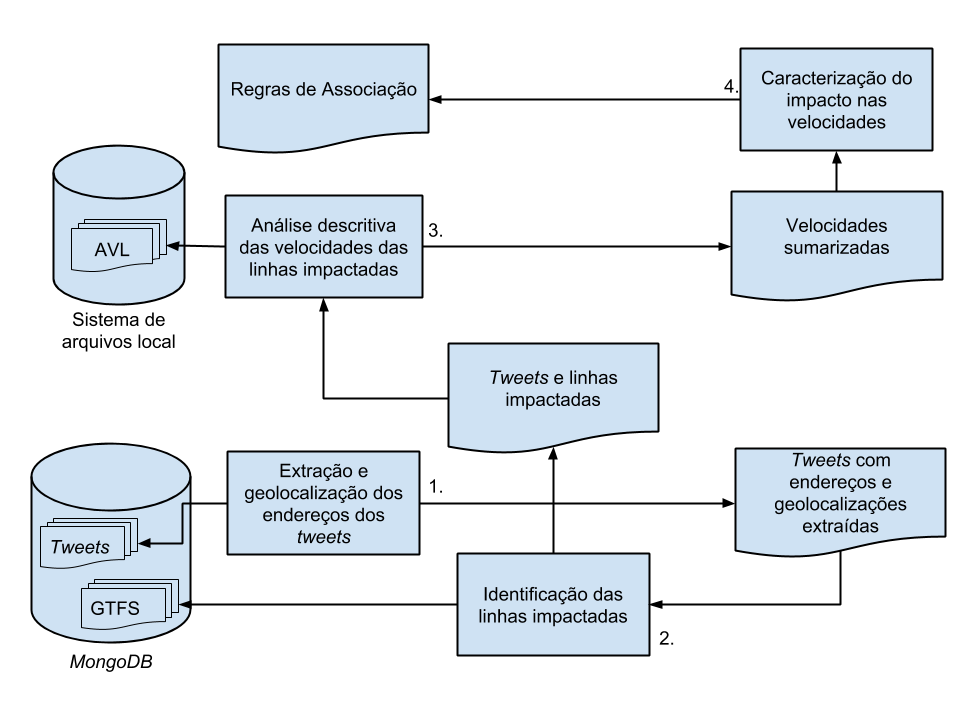
\includegraphics[width=0.9\linewidth]{caracterization_flow.png}
\end{figure}
\end{frame}
%------------------------------------------------
\section{Exploração e visualização de grandes volumes de dados}
\begin{frame}
\Huge{\centerline{Exploração e visualização}}
\Huge{\centerline{de grandes volumes de dados}}
\end{frame}
%------------------------------------------------
%\subsection{Correlação dos eventos de exceção com os dados AVL da SPTrans}
%\begin{frame}
%\frametitle{Correlação dos eventos de exceção com os dados AVL da SPTrans}
%\begin{itemize}
%\item Atraso médio induzido nas viagens.
%\item Ônibus frequentemente afetados por eventos de exceção.
%\item Ônibus frequentemente afetados por determinado evento de exceção.
%\item Padrão de ocorrência dos eventos de exceção no espaço-tempo (localizações e \textit{timestamps}).
%\item Quantidade e viagens afetadas.
%\item Quantidade e regiões da cidade de São Paulo afetadas.
%\item Viagens frequentemente afetadas por eventos de exceção.
%\item Viagens frequentemente afetadas por determinado evento de exceção.
%\end{itemize}
%\end{frame}
%------------------------------------------------
\begin{frame}{Exploração e visualização de grandes volumes de dados}
\begin{block}{Trabalhos relacionados}
\begin{itemize}
\item Apresentação de conceitos básicos e fluxos de visualização de dados de tráfego (dos dados brutos, pré-processamento ao mapeamento visual, construído com símbolos visuais). Técnicas e métodos de processamento de dados para descrever propriedades temporais, espaciais, numéricas e categóricas de dados de tráfego.
\item Descrição de uma tipologia de dados de tráfego, capaz de abordar suas respectivas propriedades, problemas e transformações relevantes para a análise. Abordagens analíticas visuais para analisar dados de tráfego de veículos, pedestres, passageiros dentro de sistemas de transporte, etc.
\item Apresentação de um novo algoritmo para mapeamento de medições coletivas para monitorar as infraestruturas de transporte terrestre e, aliviar o impacto de imprecisões do GPS para monitoramento contínuo de infraestruturas de transporte por meio de \textit{smart phones}.
\end{itemize}
\end{block}
\end{frame}
%------------------------------------------------
\begin{frame}{Exploração e visualização de grandes volumes de dados}
\begin{block}{Definição}
São cidades sustentáveis e socialmente inclusivas, que utilizam Tecnologias da Informação e Comunicação (TICs) para gerir eficientemente seus respectivos recursos naturais.
\end{block}
\begin{block}{Desafios}
    \begin{itemize}
        \item \alert{Conectividade:} Infraestrutura de redes, interoperabilidade, escalabilidade, tolerância a falhas, etc.
        \item \alert{Data:} Capacidade de armazenamento e localização dos dados, extração, processamento, análise, exploração e visualização; correlação de dados de fontes heterogêneas, processamento em tempo real, etc.
    \end{itemize}
\end{block}
\end{frame}
\subsection{Arquitetura proposta}
\begin{frame}
\frametitle{Arquitetura proposta}
\begin{block}{Druid}
\begin{itemize}
    \item O Druid é um banco de dados para análises exploratórias em tempo real (latências abaixo de sub-segundos) em grandes conjuntos de dados.
    \item Arquitetura distribuída composta por um cluster com diferentes tipos de nós (real- time, historical, broker e coordinator nodes).
    \item Nós independentementes uns dos outros e possuem interação mínima entre eles. 
    \item Dependências externas: (I) Apache Zookeeper1, responsável pela coordenação do cluster e (II) um sistema de gerenciamento de banco de dados relacional (RDBMS — Relational Data- base Management Systems), para armazenar parâmetros operacionais adicionais e configurações.
\end{itemize}
\end{block}
\end{frame}
\begin{frame}
\frametitle{Arquitetura proposta}
\begin{block}{Apache Superset}
Aplicação web para exploração e visualização de dados.
\end{block}
\begin{block}{Apache Kafka}
Aplicação para processamento de fluxos de dados em quase tempo real.
\end{block}
\begin{figure}[!htb]% H manda colocar exatamente nessa posição no texto (relativa aos parágrafos anterior e posterior)
	\centering
 	  \caption{Arquitetura utilizada no estudo de caso}
		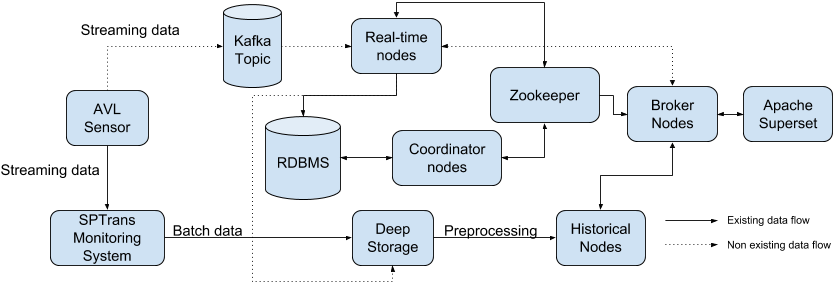
\includegraphics[width=0.9\linewidth]{viz_arch_en.png}
	\label{fig:viz_arch}
%  \source{Felipe Cordeiro Alves Dias, 2017}
\end{figure}
\end{frame}
%------------------------------------------------
\begin{frame}
\frametitle{Arquitetura proposta}
\framesubtitle{Real-time nodes}
\alert{Real-time nodes}
\begin{itemize}
\item Ingerir, indexar e consultar fluxos de eventos. 
\item Periodicamente, cada nó agenda uma tarefa em segundo plano para procurar todos os índices localmente persistidos, mesclando-os para construir blocos imutáveis de dados com todos os eventos ingeridos em um período de tempo.
\item Segmentos imutáveis: podem posteriormente serem carregados para uma camada de sistema de arquivos (deep storage).
\item Não há perda de dados e a imutabilidade dos blocos permite a consistência de leitura e um modelo de paralelização simples: \textit{historical nodes} podem simultaneamente examinar e agregar blocos imutáveis de forma não bloqueante.
\end{itemize}
\end{frame}
\begin{frame}
\frametitle{Arquitetura proposta}
\framesubtitle{Historical, broker and coordinator nodes}
\begin{itemize}
    \item \alert{Historical nodes}: Os historical nodes são responsáveis por carregar, descartar e servir segmentos imutáveis por meio de uma arquitetura shared-nothing (sem um único ponto de contenção entre os nós).
    \item\alert{Broker nodes}: Os broker nodes são responsáveis por receber consultas e mesclar resultados parciais dos historicals e real-time nodes antes de retornar um resultado final consolidado para o cliente.
    \item \alert{Coordinator nodes}: Os coordinator nodes são responsáveis pelo gerenciamento e distribuição dos dados nos historical nodes, exigindo destes o carregamento, descarte e replicação dos dados.
\end{itemize}
\end{frame}
%------------------------------------------------
\subsection{Validação da arquitetura proposta}
\begin{frame}
\frametitle{Validação da arquitetura proposta}
\framesubtitle{Quantidade de dados enviados por dia por ônibus (selecionados aleatoriamente) em janeiro de 2017}
\begin{figure}[!htb]% H manda colocar exatamente nessa posição no texto (relativa aos parágrafos anterior e posterior)
	\centering
		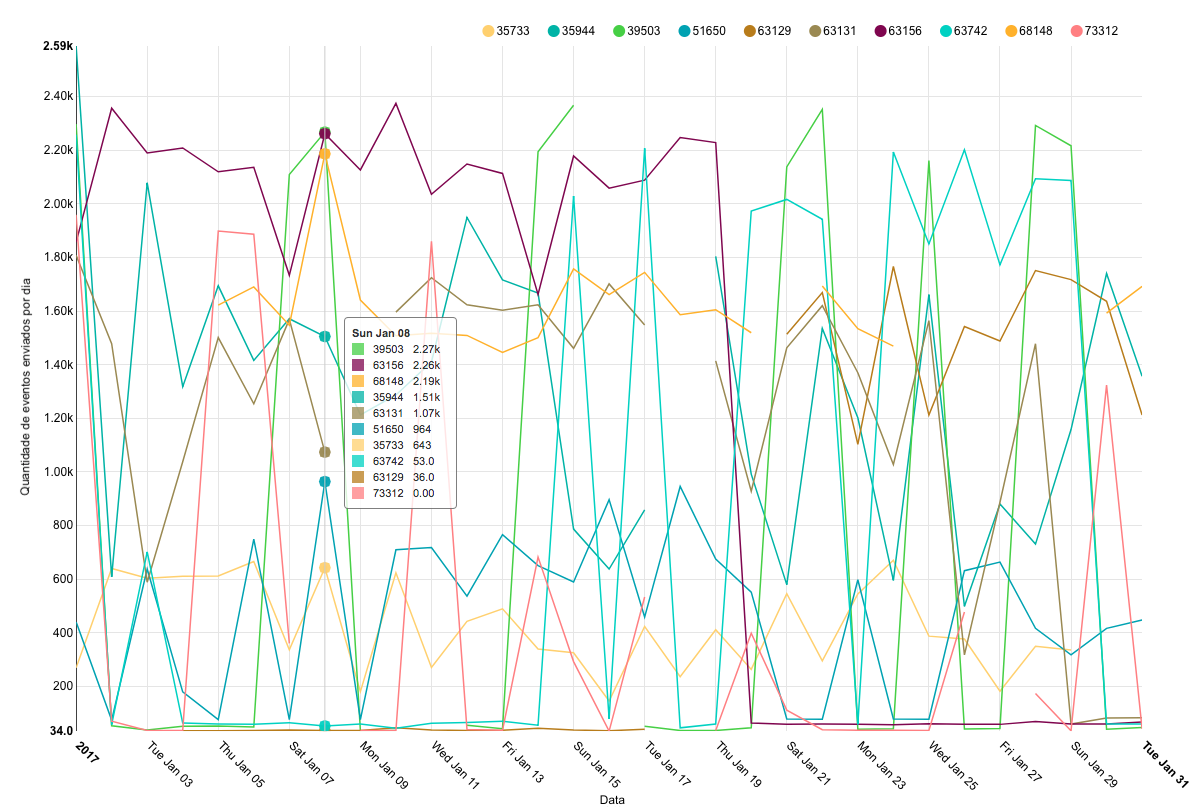
\includegraphics[width=0.90\linewidth]{analysis_by_bus_lines_pt.png}
	\label{fig:only_one_bus_map}
  %\source{Felipe Cordeiro Alves Dias, 2017}
\end{figure}
\end{frame}
\begin{frame}
\frametitle{Validação da arquitetura proposta}
\framesubtitle{Distribuição da quantidade de dados enviados por ônibus (selecionados aleatoriamente) em janeiro de 2017}
\begin{figure}[!htb]% H manda colocar exatamente nessa posição no texto (relativa aos parágrafos anterior e posterior)
	\centering
		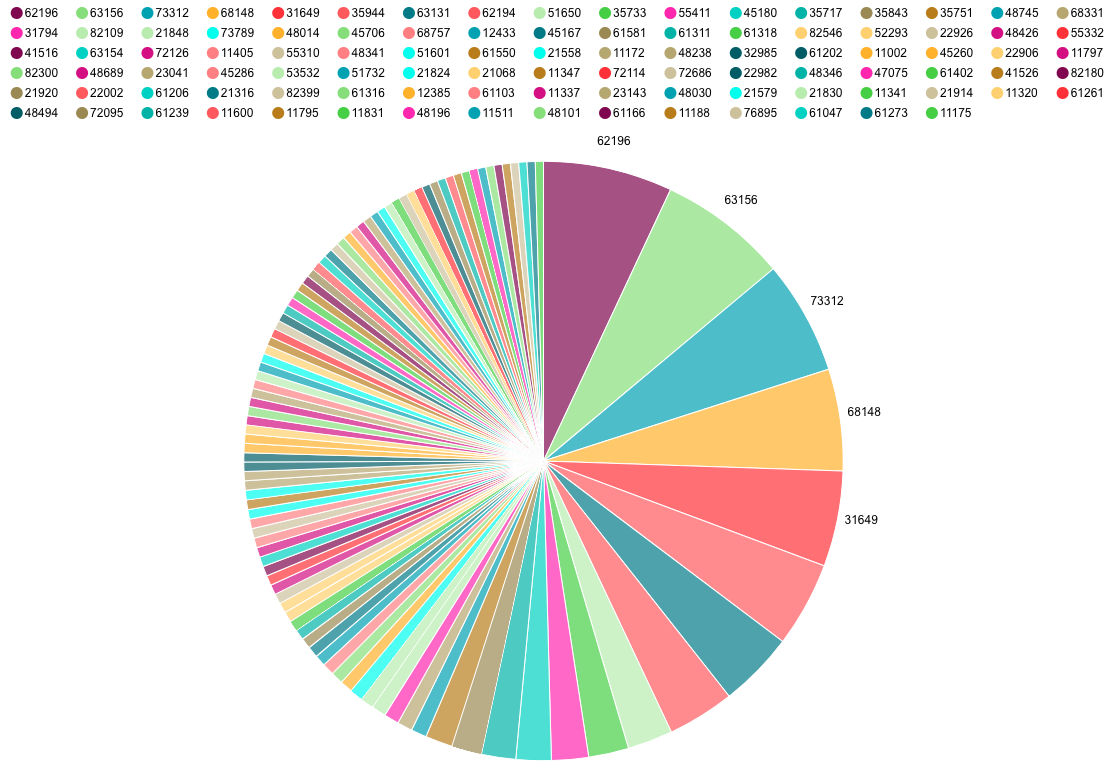
\includegraphics[width=0.85\linewidth]{pizza_bus.png}
	\label{fig:buses_map}
\end{figure}
\end{frame}
%------------------------------------------------
\begin{frame}
\frametitle{Validação da arquitetura proposta}
\framesubtitle{Localizações enviadas em Janeiro de 2017 de uma linha de ônibus selecionada aleatoriamente}
\begin{figure}[!htb]% H manda colocar exatamente nessa posição no texto (relativa aos parágrafos anterior e posterior)
	\centering
		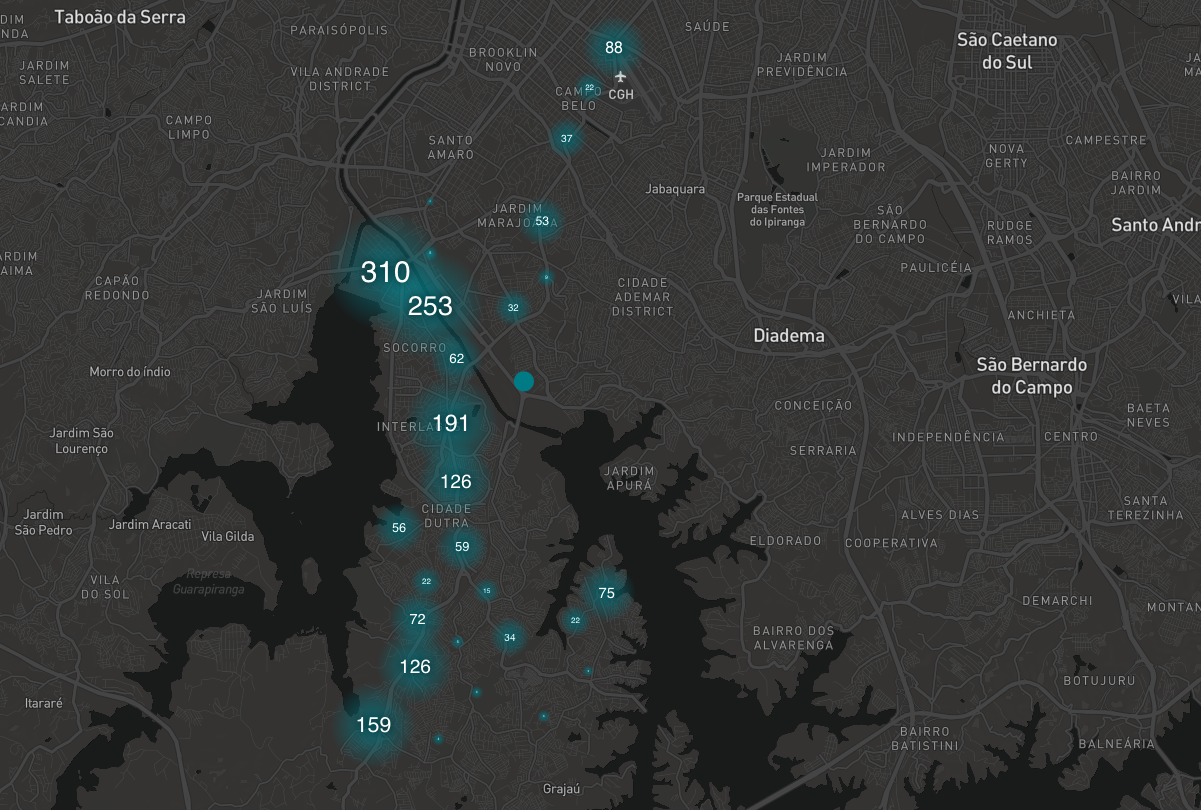
\includegraphics[width=0.85\linewidth]{only_one_bus_map.png}
	\label{fig:analysis_by_bus_lines}
  %\source{Felipe Cordeiro Alves Dias, 2017}
\end{figure}
\end{frame}
%------------------------------------------------
\begin{frame}
\frametitle{Validação da arquitetura proposta}
\framesubtitle{Localizações dos ônibus referente a movimentação de Janeiro de 2017}
\begin{figure}[!htb]% H manda colocar exatamente nessa posição no texto (relativa aos parágrafos anterior e posterior)
	\centering
		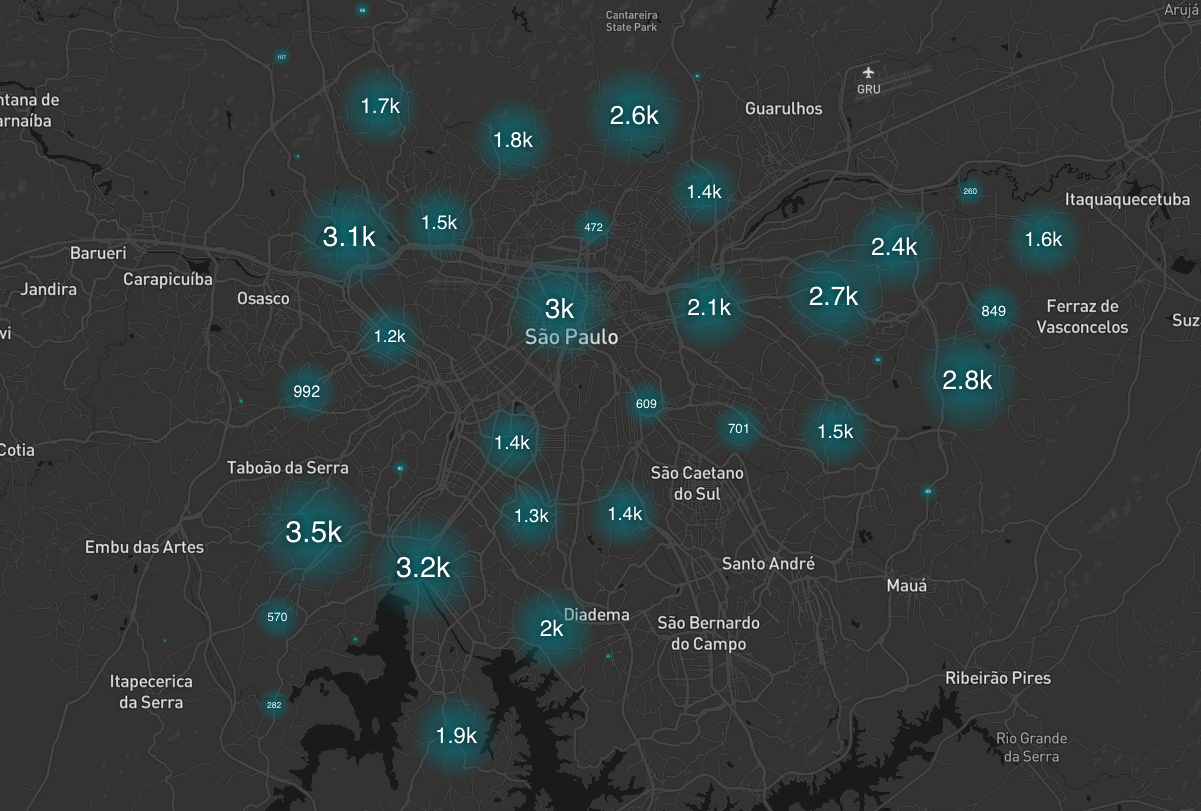
\includegraphics[width=0.90\linewidth]{buses_map.png}
	\label{fig:pizza_bus}
  %\source{Felipe Cordeiro Alves Dias, 2017}
\end{figure}
\end{frame}
%------------------------------------------------
\begin{frame}{Consideração sobre a arquitetura utilizada para exploração e visualização dos dados AVL da SPTrans}
\begin{itemize}
    \item Eestudo de caso relacionado à visualização de grandes conjuntos de dados, utilizando dados dos ônibus da cidade de São Paulo. 
    \item Mostramos que é possível encontrar padrões complexos e incomuns e possíveis eventos de exceção em grandes conjuntos de dados por meio da visualização. 
    \item O Druid e o Apache Superset demonstraram suporte a agregação, exploração e visualização de grandes conjuntos de dados.
\end{itemize}
\end{frame}
%------------------------------------------------
\section{Mineração e geolocalização automatizada de eventos de exceção a partir de dados do Twitter}
\begin{frame}
\Huge{\centerline{Mineração e geolocalização}}
\Huge{\centerline{automatizada de eventos de exceção}}
\Huge{\centerline{a partir de dados do \textit{Twitter}}}
\end{frame}
%------------------------------------------------
\begin{frame}{Mineração e geolocalização automatizada de eventos de exceção a partir de dados do \textit{Twitter}}
    \begin{figure}[!htb]% H manda colocar exatamente nessa posição no texto (relativa aos parágrafos anterior e posterior)
	\centering
		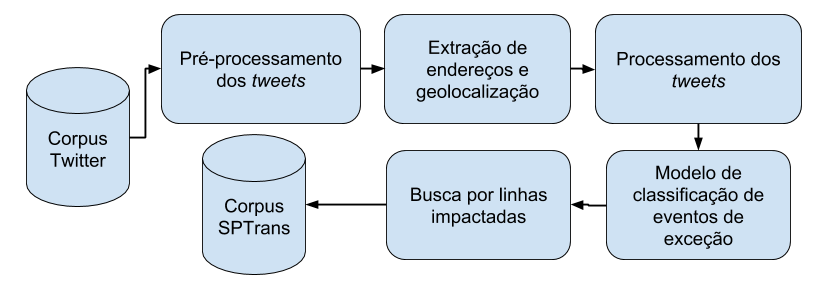
\includegraphics[width=1\linewidth]{tweet_based_methodology_pt.png}
	\label{fig:pizza_bus}
  %\source{Felipe Cordeiro Alves Dias, 2017}
\end{figure}
Expressão regular para extração de endereços:
\begin{equation}
ER = \lbrace L_1 | S_1 | L_2 | S_2 | \dots | L_n | S_n \rbrace \lbrace [a-z\grave{A}-\ddot{y}\_] + \rbrace
\end{equation}
Geolocalização dos endereços usando a API do Google Geocoding.
\end{frame}
%------------------------------------------------
\begin{frame}{Resultados da classificação, manual, pré-processamento, processamento dos tweets e extração de endereços}
\begin{itemize}
    \item No final do pré-processamento e processamento dos tweets, o corpus obteve 414,637 palavras, com um vocabulário de 13,915 palavras. O comprimento máximo das sentenças do conjunto de dados é 19.
    \item 60.984 \textit{tweets} classificados manualmente.
    \item Dos 60.984 tweets, 10.027 foram classificados manualmente em eventos de exceção e desse subconjunto foram encontrados 8.112 endereços. Desconsiderando o tipo de localidade APPROXIMATE (explicado mais adiante) --- (o que representa 80,90\% do total dos tweets classificados como eventos de exceção, sem considerar a classe Irrelevante).
\end{itemize}
\end{frame}
%------------------------------------------------
\begin{frame}{Resultado da distribuição das classes dos eventos de exceção do Corpus Twitter}
\begin{figure}[!htb]% H manda colocar exatamente nessa posição no texto (relativa aos parágrafos anterior e posterior)
	\centering
		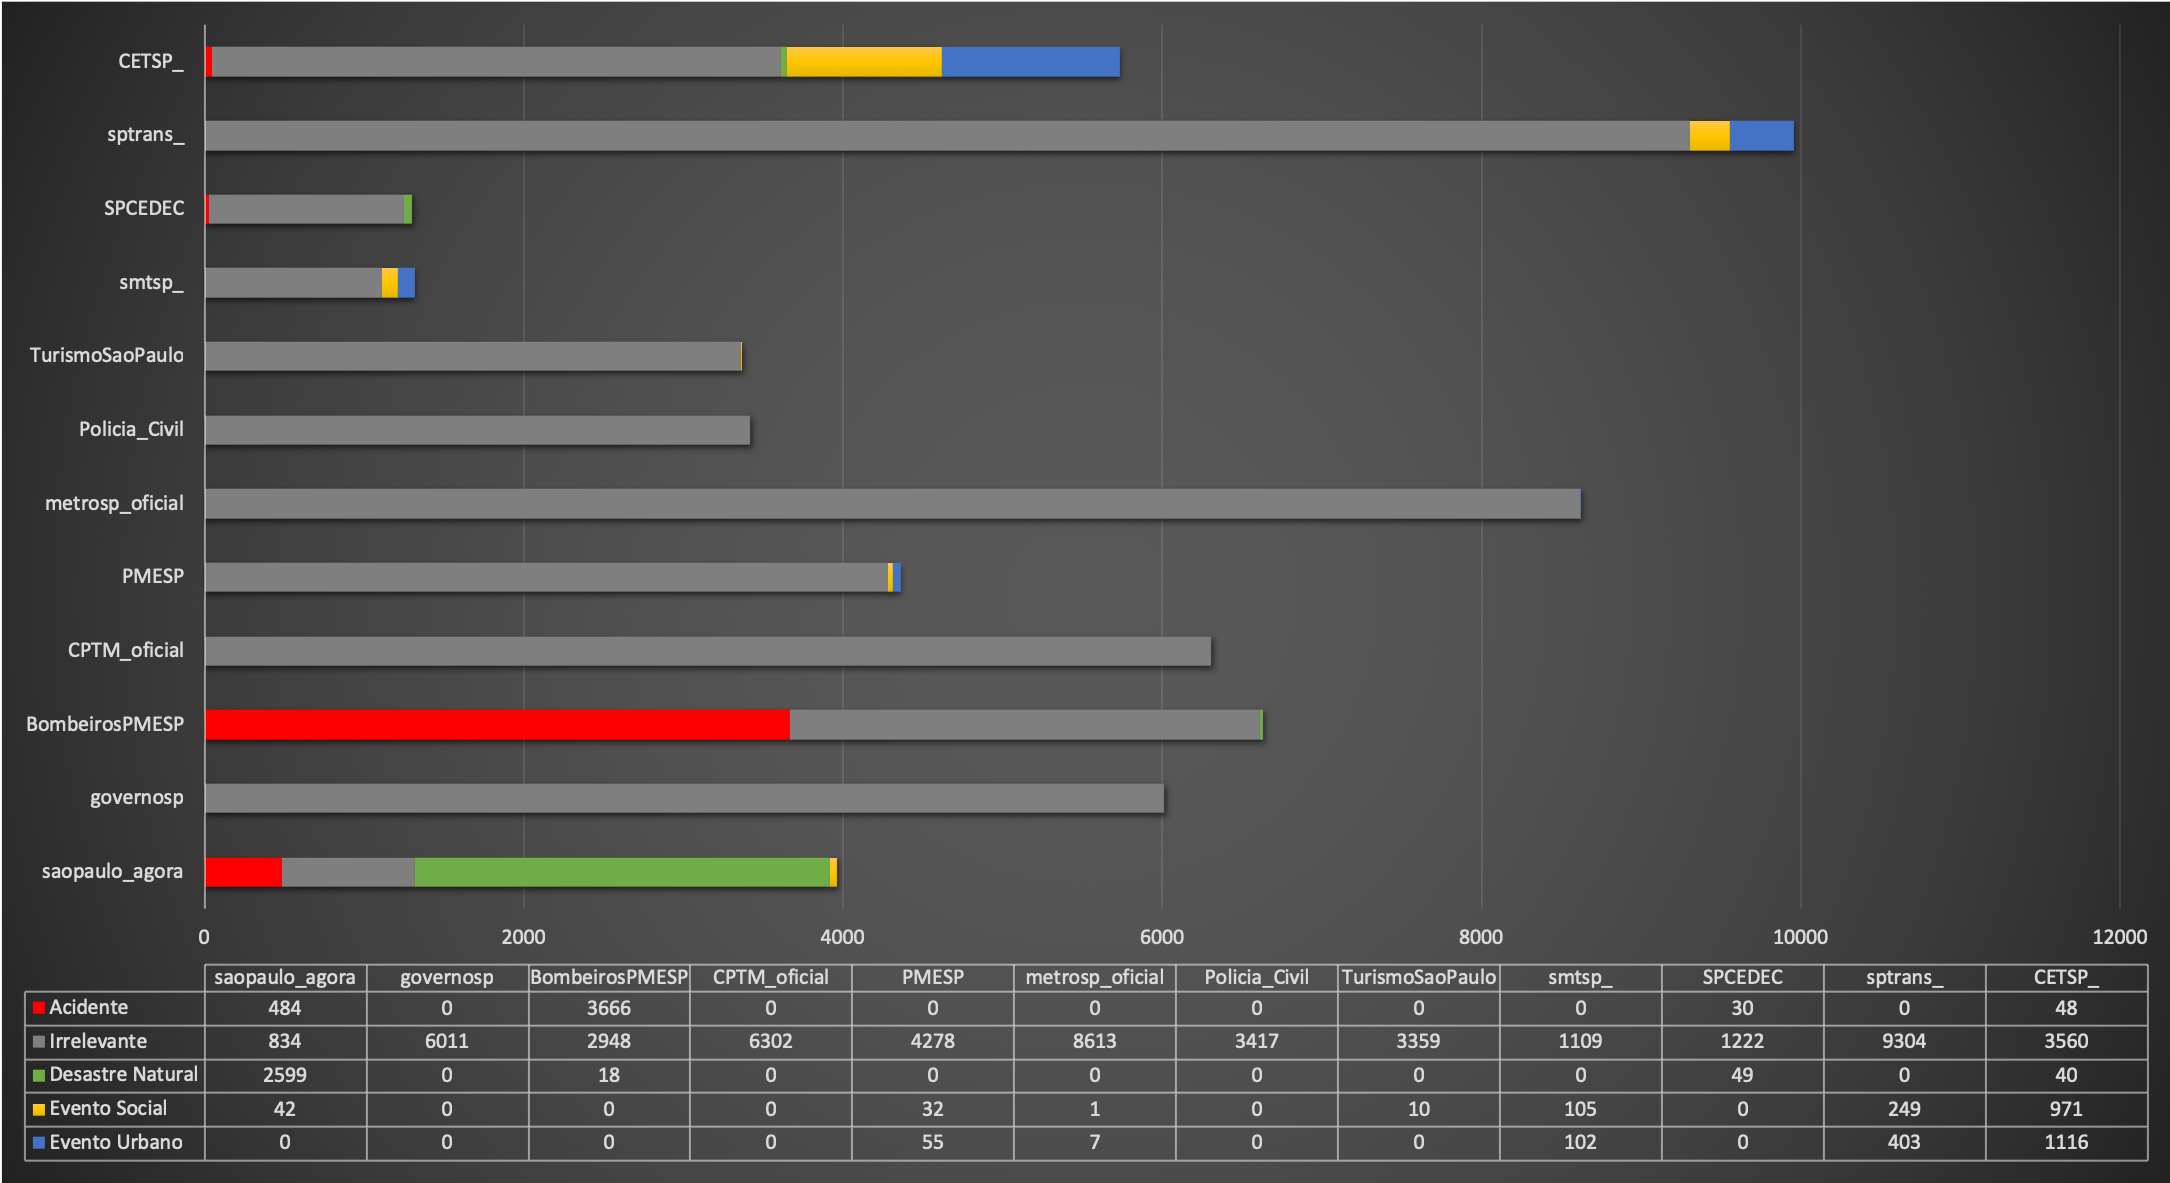
\includegraphics[width=1\linewidth]{tweets_distribution_pt.png}
	\label{fig:pizza_bus}
  %\source{Felipe Cordeiro Alves Dias, 2017}
\end{figure}
\end{frame}
%------------------------------------------------
\begin{frame}{Resultados dos modelos para classificação automatizada dos eventos de exceção}
\begin{table}[!htb]
\centering
\caption {Métricas das avaliações dos algoritmos utilizados para classificação dos \textit{tweets} em eventos de exceção}
\label {tab:metrics}
\begin{tabular}{c|c|c|c|c}
\toprule
\textbf{Algoritmo} & \textbf{ACC} & \textbf{PPV} & \textbf{TPR} & \textbf{\textit{f1-score}} \\
\midrule
\textit{Naive Bayes} Complementar & 0,941 & 0,949 & 0,941 & 0,944 \\
\hline
Árvore de Decisão & 0,965 & 0,965 & 0,965 & 0,965 \\
\hline
K-ésimo Vizinho mais Próximo & 0,970 & 0,971 & 0,970 & 0,970 \\
\hline
Regressão Logística & 0,969 & 0,968 & 0,969 & 0,968 \\
\hline
Perceptron multicamadas & \textit{0,973} & \textit{0,972} & \textit{0,973} & \textit{0,972} \\
\hline
\textit{Naive Bayes} Multinomial & 0,953 & 0,952 & 0,953 & 0,949 \\
\hline
Floresta Aleatória & 0,970 & 0,970 & 0,970 & 0,970 \\
\hline
Máquina de Vetores de Suporte & 0,833 & 0,694 & 0,833 & 0,757 \\
\bottomrule
\end{tabular}
%\source{Felipe Cordeiro Alves Dias, 2019}
\end{table}
\end{frame}
%------------------------------------------------
\begin{frame}{Resultados da matriz de confusão do modelo Perceptron multicamadas}
\begin{figure}[!htb]% H manda colocar exatamente nessa posição no texto (relativa aos parágrafos anterior e posterior)
	\centering
		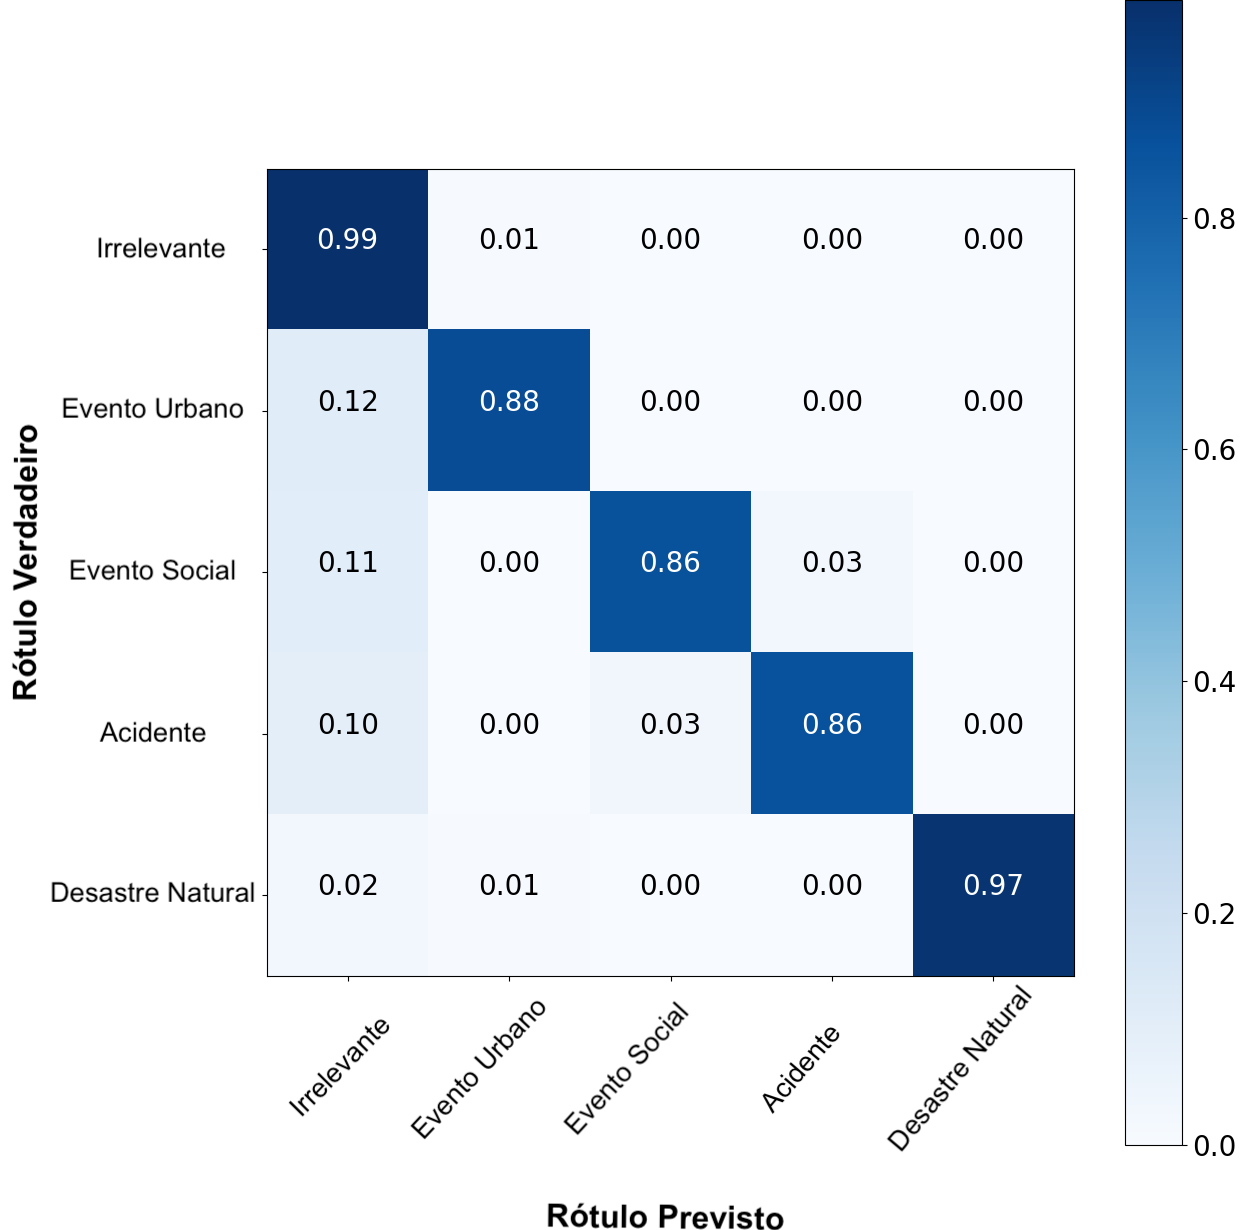
\includegraphics[width=0.7\linewidth]{confusion_matrix_mlp_pt.png}
	\label{fig:pizza_bus}
  %\source{Felipe Cordeiro Alves Dias, 2017}
\end{figure}
\end{frame}
%------------------------------------------------
\begin{frame}{Resultados da distribuição de endereços extraídos por classe}
\begin{table}[!htb]
\centering
\caption {Quantidade\tnote{f} de endereços extraídos por classe}
\label {tab:qtdExtractedAddresses}
\begin{adjustbox}{max height=10mm, width=4in}
\begin{threeparttable}
\begin{tabular}{c|c|c|c|c|c}
\toprule
\textbf{Classe} & \textbf{\#endereços extraídos\tnote{a}} & \textbf{\textit{\#APP\tnote{b}}} & \textbf{\textit{\#GEO\tnote{c}}} & \textbf{\textit{\#RANGE\tnote{d}}} & \textbf{\textit{\#ROOF\tnote{e}}} \\
\midrule
Acidente & 3.439 & 7 & 805 & 1.130 & 1.497 \\
\hline
Irrelevante & 451 & 13 & 292 & 6 & 140 \\
\hline
Desastre Natural & 2.464 & 9 & 340 & 719 & 1.396 \\
\hline
Evento Social & 793 & 4 & 761 & 2 & 26 \\
\hline
Evento Urbano & 1.002 & 4 & 942 & 10 & 46 \\
\midrule
\midrule
\textbf{Total} & 8.149 & 37 & 3.140 & 1.867 & 3.105 \\
\bottomrule
\end{tabular}
\begin{tablenotes}
\item[a] Total de endereços extraídos
\item[b] Total de endereços extraídos com o tipo de localidade \textit{APPROXIMATE}
\item[c] Total de endereços extraídos com o tipo de localidade \textit{GEOMETRIC\_CENTER}
\item[d] Total de endereços extraídos com o tipo de localidade \textit{RANGE\_INTERPOLATED}
\item[e] Total de endereços extraídos com o tipo de localidade \textit{ROOFTOP}
\item[f] Total considerando endereços repetidos, a repetição é importante para identificarmos os endereços mais impactados por eventos de exceção.
\end{tablenotes}
\end{threeparttable}
\end{adjustbox}
\end{table}
\end{frame}
%------------------------------------------------
\begin{frame}{Resultados da distribuição de endereços extraídos por classe}
Os \textit{tipos de localidades}\footnote{Disponível em \url{https://developers.google.com/maps/documentation/geocoding}. Acesso em 16 de setembro de 2018.} são classificados pela \textit{Google Geocoding API} em:
\begin{enumerate}
\item \textit{ROOFTOP} --- Indica que o resultado retornado há informações de localização com precisão a nível do endereço de rua.
\item \textit{RANGE\_INTERPOLATED} --- Indica que o resultado retornado reflete uma aproximação interpolada entre dois pontos precisos (como interseções). Geralmente, os resultados interpolados são retornados quando os códigos geográficos do \textit{rooftop} não estão disponíveis para um endereço de rua.
\item \textit{GEOMETRIC\_CENTER} --- Indica que o resultado retornado é o centro geométrico de um resultado.
\item \textit{APPROXIMATE} --- Indica que o resultado retornado é aproximado.
\end{enumerate}
\end{frame}
%------------------------------------------------
\begin{frame}{Resultados da distribuição de endereços extraídos por classe}
\begin{enumerate}
\item \textit{Tweets} apenas com o ponto de interesse, ou seja, não consta explicitamente o endereço.
\item \textit{Tweets} sem informação de endereço.
\item \textit{Tweets} com nome de logradouro incomum (por exemplo \emph{passagem}, \emph{complexo viário}, \emph{ligação sentido}).
\item \textit{Tweets} com endereços com palavras concatenadas (por exemplo \emph{avenidapaulista}).
\end{enumerate}
\end{frame}
%------------------------------------------------
\begin{frame}{Resultado da análise visual da distribuição dos eventos de exceção na região central de São Paulo}
\begin{figure}[!htb]% H manda colocar exatamente nessa posição no texto (relativa aos parágrafos anterior e posterior)
	\centering
		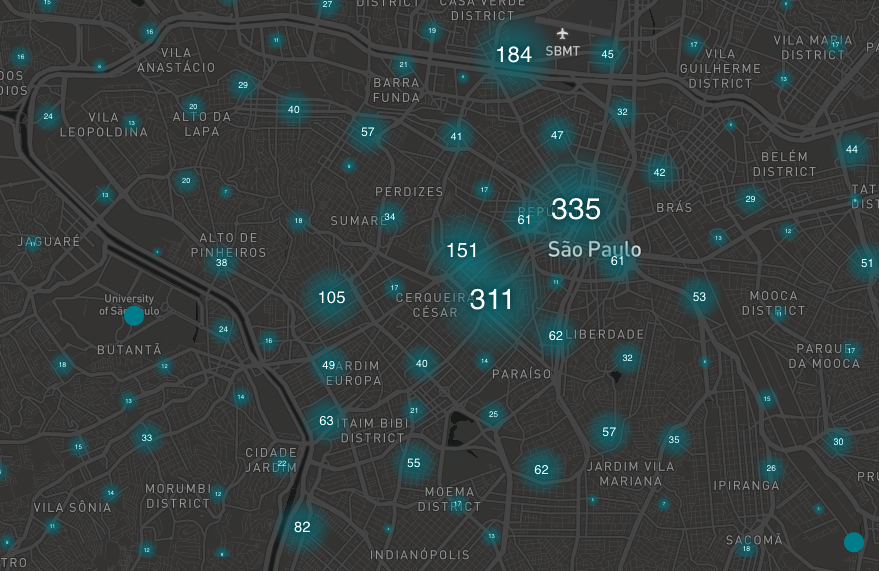
\includegraphics[width=1\linewidth]{exception_events_sp.png}
	\label{fig:pizza_bus}
  %\source{Felipe Cordeiro Alves Dias, 2017}
\end{figure}
\end{frame}
%------------------------------------------------
\begin{frame}{Resultado dos endereços mais impactados por eventos de exceção}
    \begin{figure}[!htb]% H manda colocar exatamente nessa posição no texto (relativa aos parágrafos anterior e posterior)
	\centering
		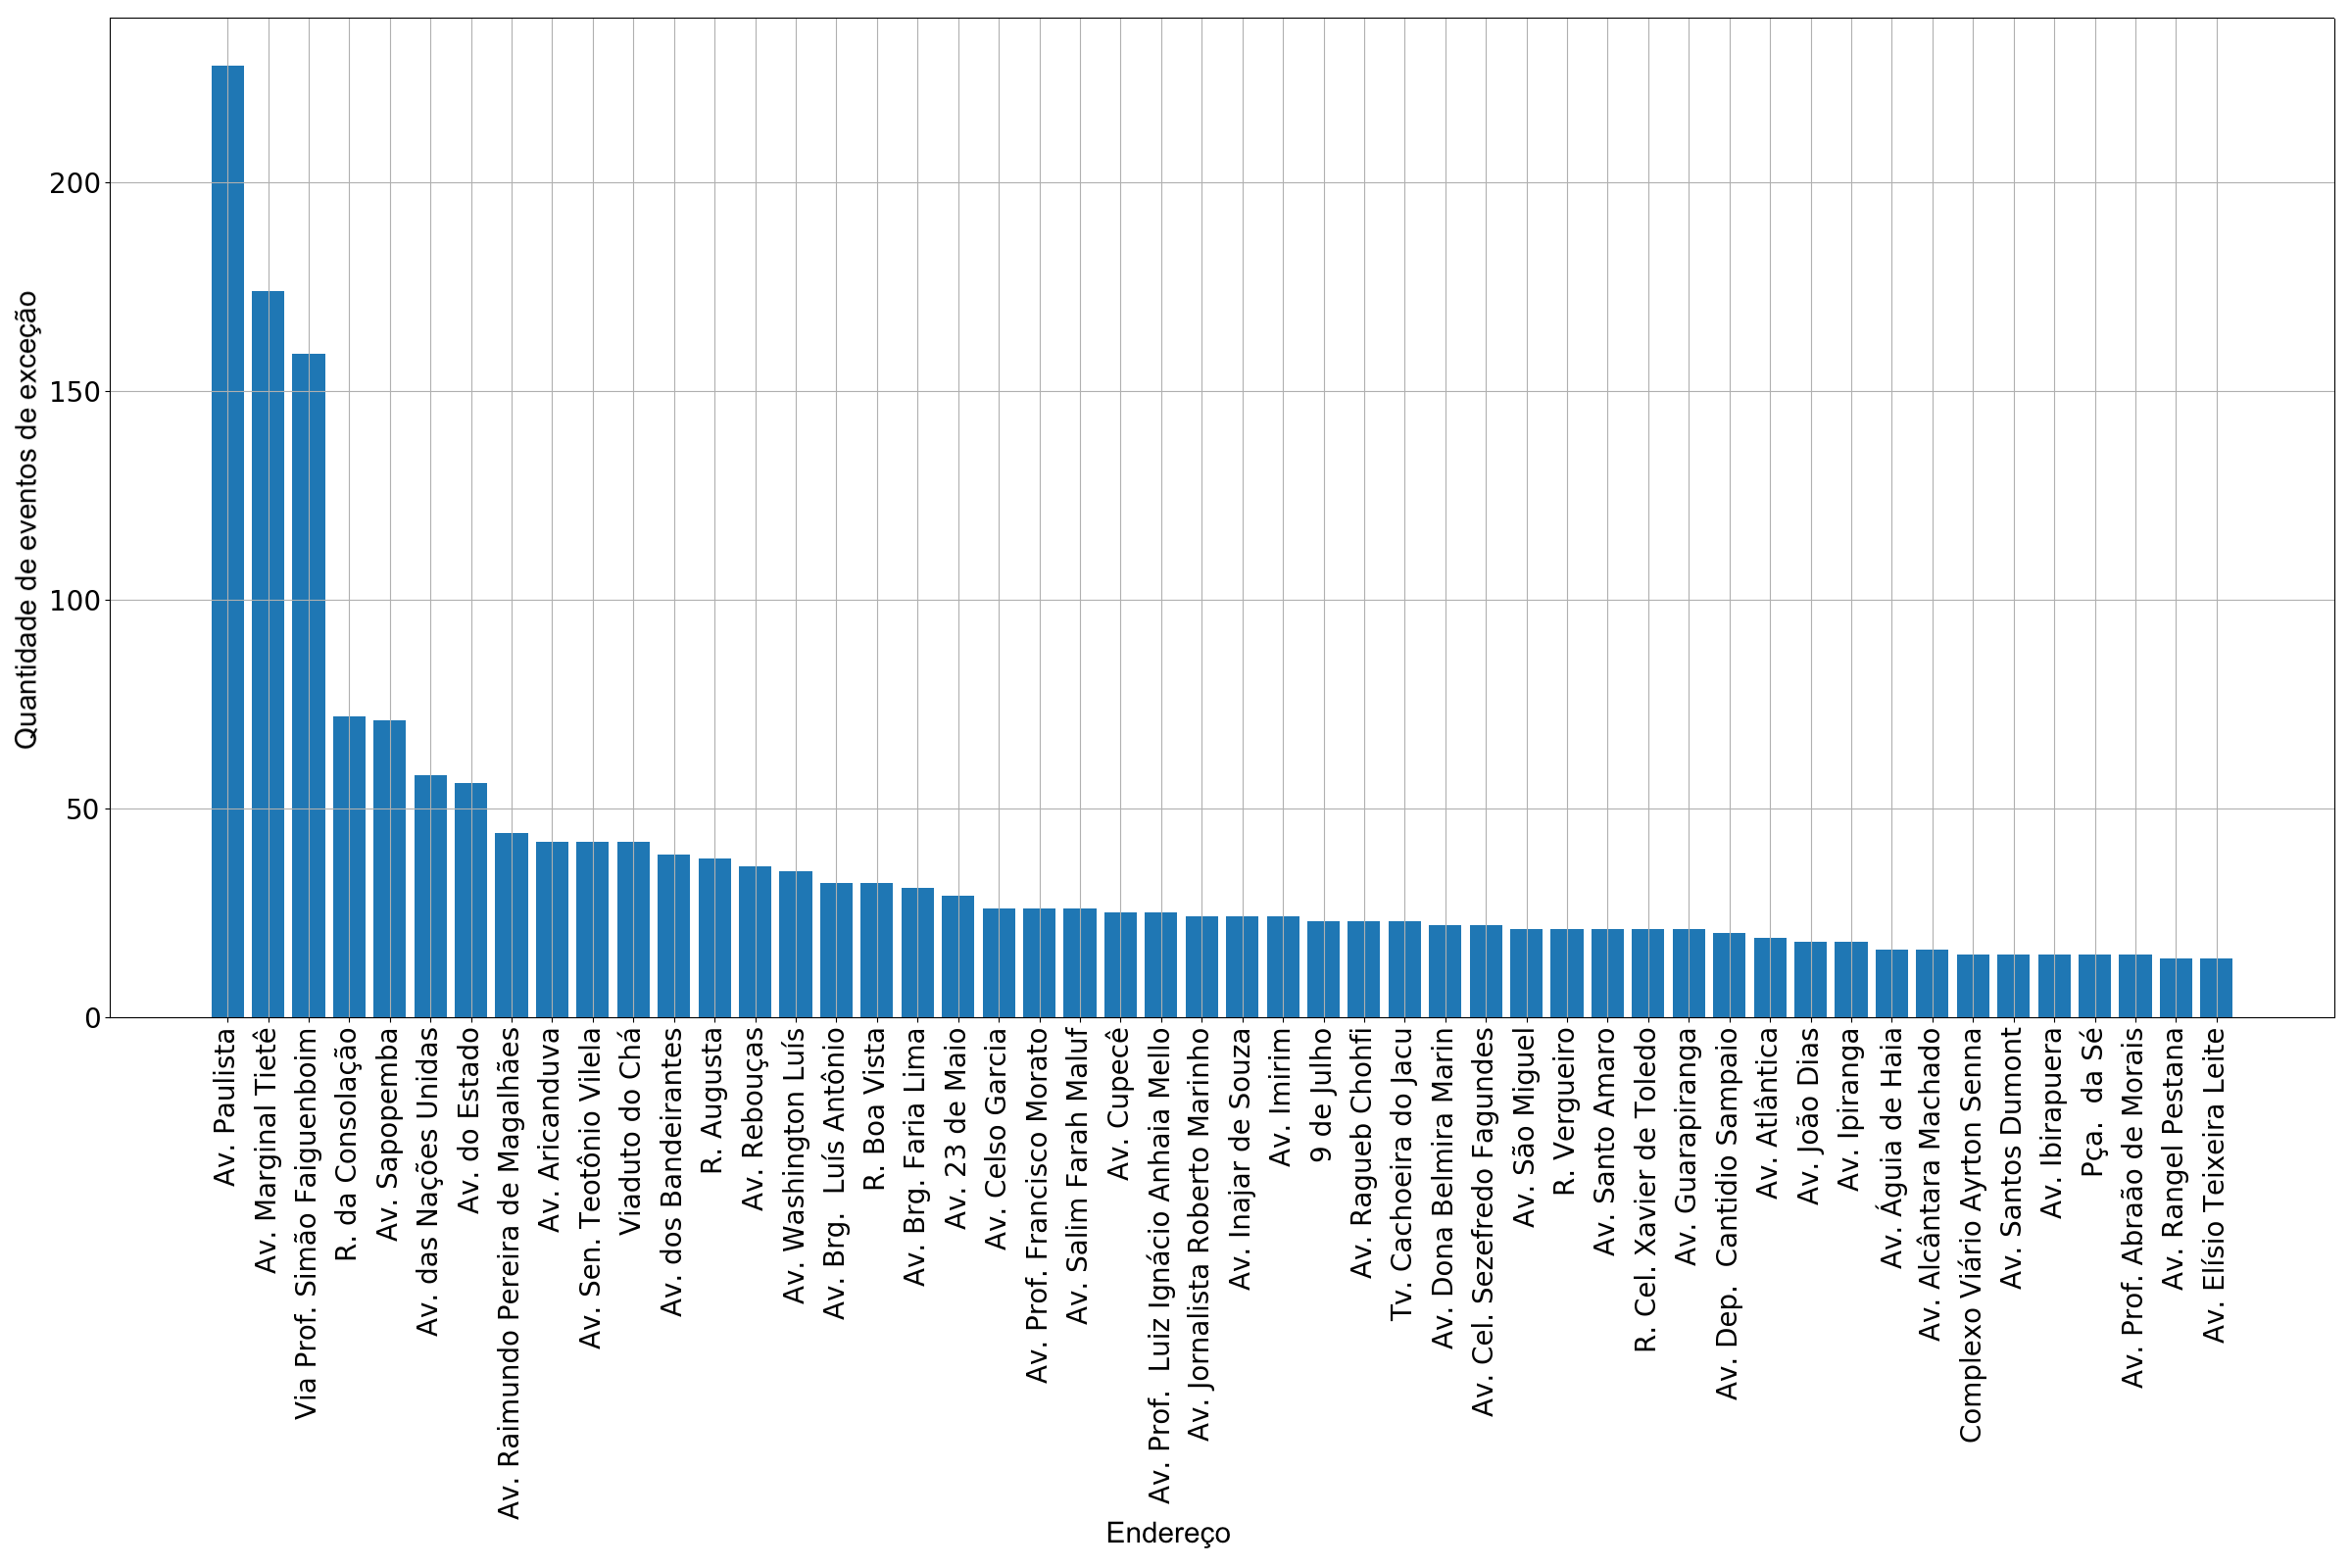
\includegraphics[width=1\linewidth]{address_analysis_pt.png}
	\label{fig:pizza_bus}
  %\source{Felipe Cordeiro Alves Dias, 2017}
\end{figure}
\end{frame}
%------------------------------------------------
\begin{frame}{Resultados das linhas de ônibus mais impactadas por eventos de exceção}
\begin {table} [!htb]
\centering
\begin{adjustbox}{max height=10mm, width=4in}
\begin{threeparttable}
\caption {Linhas de ônibus mais impactadas por eventos de exceção\tnote{a}}
\label {tab:impacted_bus_code_lines}
\begin {tabular} {c|c|c}
 \toprule
\textbf{Código da linha} & \textbf{\# eventos de exceção} & \textbf{Letreiro} \\
    \midrule
    33389 & 1301  & TERM. PINHEIROS / METRÔ TUCURUVI  \\
\hline

    33284 & 1176  & ITAIM BIBI / METRÔ SANTANA  \\
\hline

    33121 & 1023  & TERM. PRINC. ISABEL / TERM. STO. AMARO  \\
\hline

    32805 & 1006  & TERM. PRINC. ISABEL / CHÁC. SANTANA  \\
\hline

    33112 & 933   & TERM. PQ. D. PEDRO II / JD. SÃO SAVÉRIO  \\
\hline

    33111 & 857   & TERM. AMARAL GURGEL / JD. DA SAÚDE  \\
\hline

    35229 & 841   & TURISMO / CIRCULAR  \\
\hline

    33443 & 816   & ANA ROSA / METRÔ SANTANA  \\
\hline

    32897 & 805   & LUZ / TERM. A. E. CARVALHO  \\
\hline

    35072 & 767   & METRÔ BARRA FUNDA / CONEXÃO PETRÔNIO PORTELA  \\
\hline

    32772 & 759   & TERM. PRINC. ISABEL / TERM. STO. AMARO  \\
\hline

    33253 & 754   & METRÔ BELÉM / JD. BONFIGLIOLI  \\
\hline

    33391 & 748   & METRÔ JABAQUARA / METRÔ SANTANA  \\
\hline

    32813 & 746   & PÇA. DA SÉ / CHÁC. SANTANA  \\
\hline

    32829 & 746   & TERM. BANDEIRA / TERM. CAPELINHA  \\
\hline

    34048 & 719   & LGO. SÃO FRANCISCO / JD. SELMA  \\
\hline

    33486 & 715   & TERM. PQ. D. PEDRO II / TERM. SÃO MATEUS  \\
\hline

    33236 & 708   & TERM. BANDEIRA / JD. JAQUELINE  \\
\hline

    33336 & 697   & PINHEIROS / IMIRIM  \\
\hline

    32816 & 693   & TERM. PQ. D. PEDRO II / TERM. STO. AMARO  \\
\hline

    33534 & 690   & CARDOSO DE ALMEIDA / MACHADO DE ASSIS  \\
\hline

    32838 & 647   & PÇA. DA SÉ / PQ. RES. COCAIA  \\
\hline

    33398 & 639   & CID. UNIVERSITÁRIA / METRÔ SANTANA  \\
\bottomrule
\end{tabular}
\begin{tablenotes}
            \item[a] Tabela completa no Apêndice~\ref{apendiceD}.
        \end{tablenotes}
\end{threeparttable}
\end{adjustbox}
\end{table}
\end{frame}
%------------------------------------------------
\begin{frame}{Considerações finais sobre a metodologia desenvolvida}
\begin{itemize}
    \item Uma nova metodologia para classificação de eventos de exceção e analisa seus respectivos impactos no sistema de transporte coletivo por ônibus da cidade de São Paulo.
    \item O algoritmo com maior  acurácia para classificação de \textit{tweets} em eventos de exceção foi \textit{Multi-layer Perceptron}.
    \item É possível extrair endereços de \textit{tweets} semi-estruturados usando apenas expressões regulares.
    \item A classificação desses eventos é o primeiro passo para entender melhor como os eventos de exceção afetam a rede de transporte público.
    \item Metodologia aplicável em diferentes idiomas e cidades (a GTFS é um formato ubíquo para o transporte público e ferramentas como a NLTK suporta vários idiomas.).
\end{itemize}
\end{frame}
%------------------------------------------------
\section{Caracterização do impacto dos eventos de exceção}
\begin{frame}
\Huge{\centerline{Caracterização do impacto}}
\Huge{\centerline{dos eventos de exceção}}
\end{frame}
%------------------------------------------------
\begin{frame}{Distribuição do número de eventos de exceção geolocalizados}
\begin{figure}[!htb]
	\centering
 	  \caption{Distribuição do número de eventos de exceção geolocalizados}
		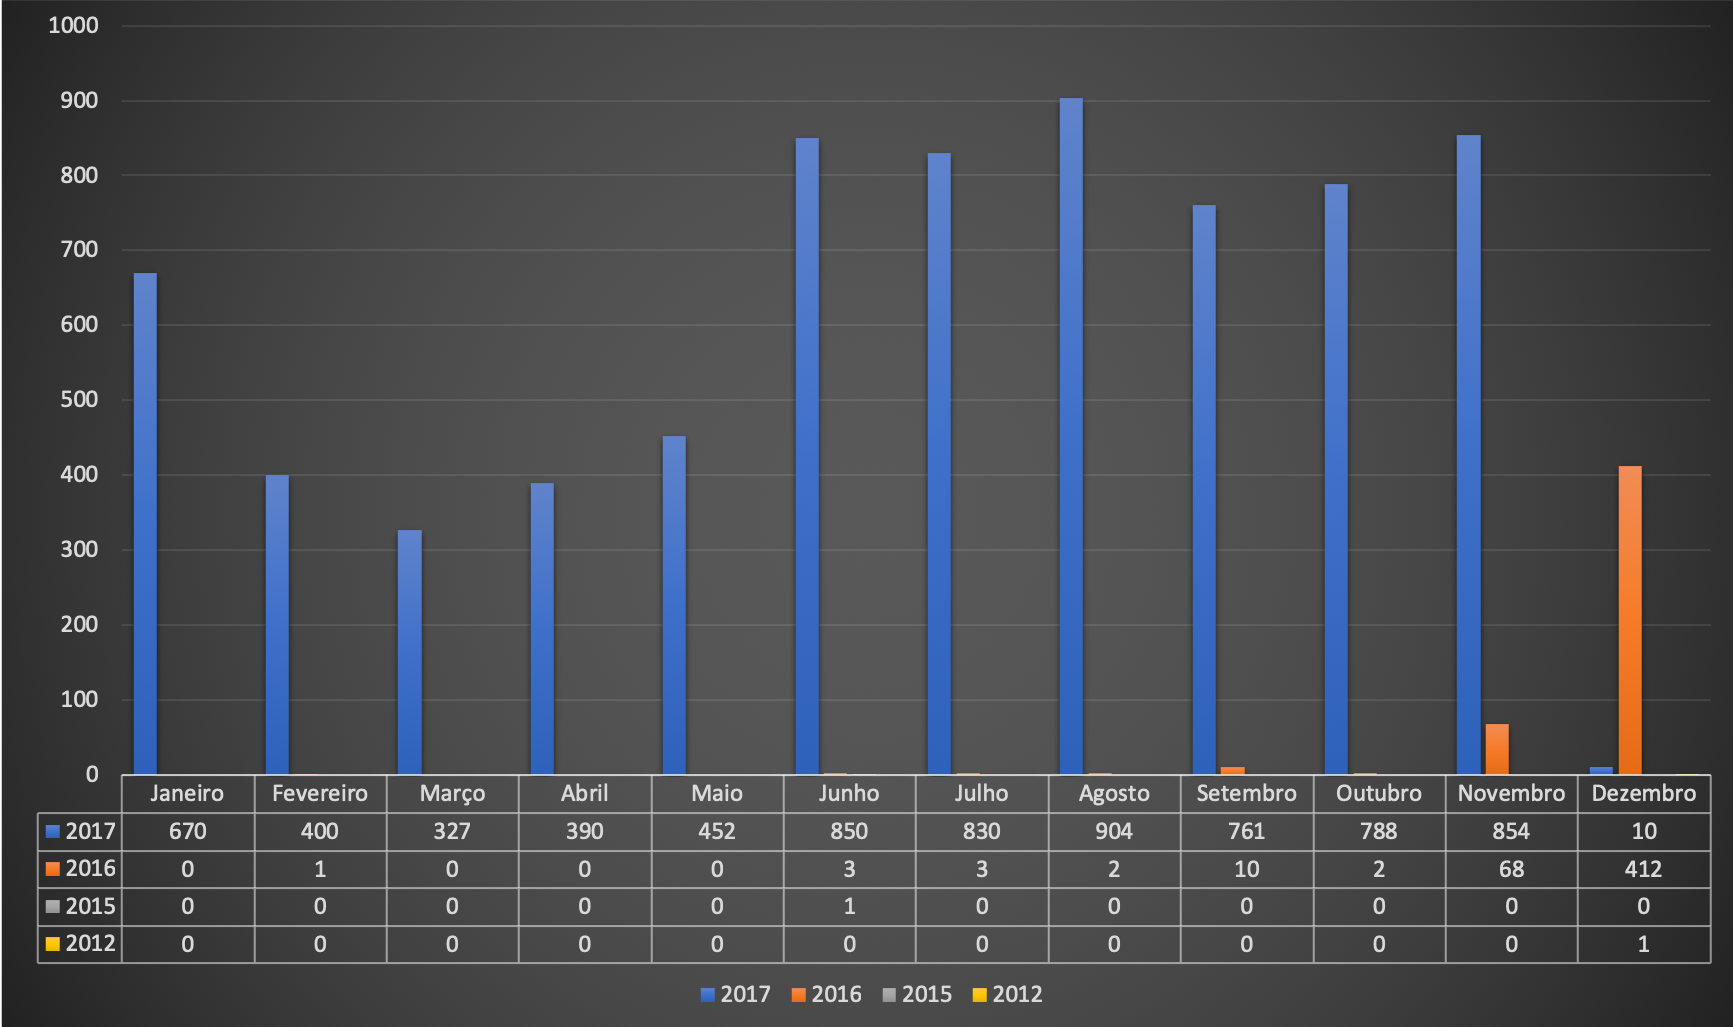
\includegraphics[width=0.8\linewidth]{geolocated_exception_events_distribution_pt.png}
	\label{fig:geolocated_exception_events_distribution}
\end{figure}
\end{frame}
%------------------------------------------------
\begin{frame}{Distribuição das classes de eventos de exceção geolocalizados ao longo dos meses do ano de 2017}
\begin{figure}[!htb]
	\centering
 	  \caption{Distribuição das classes de eventos de exceção geolocalizados ao longo dos meses do ano de 2017}
		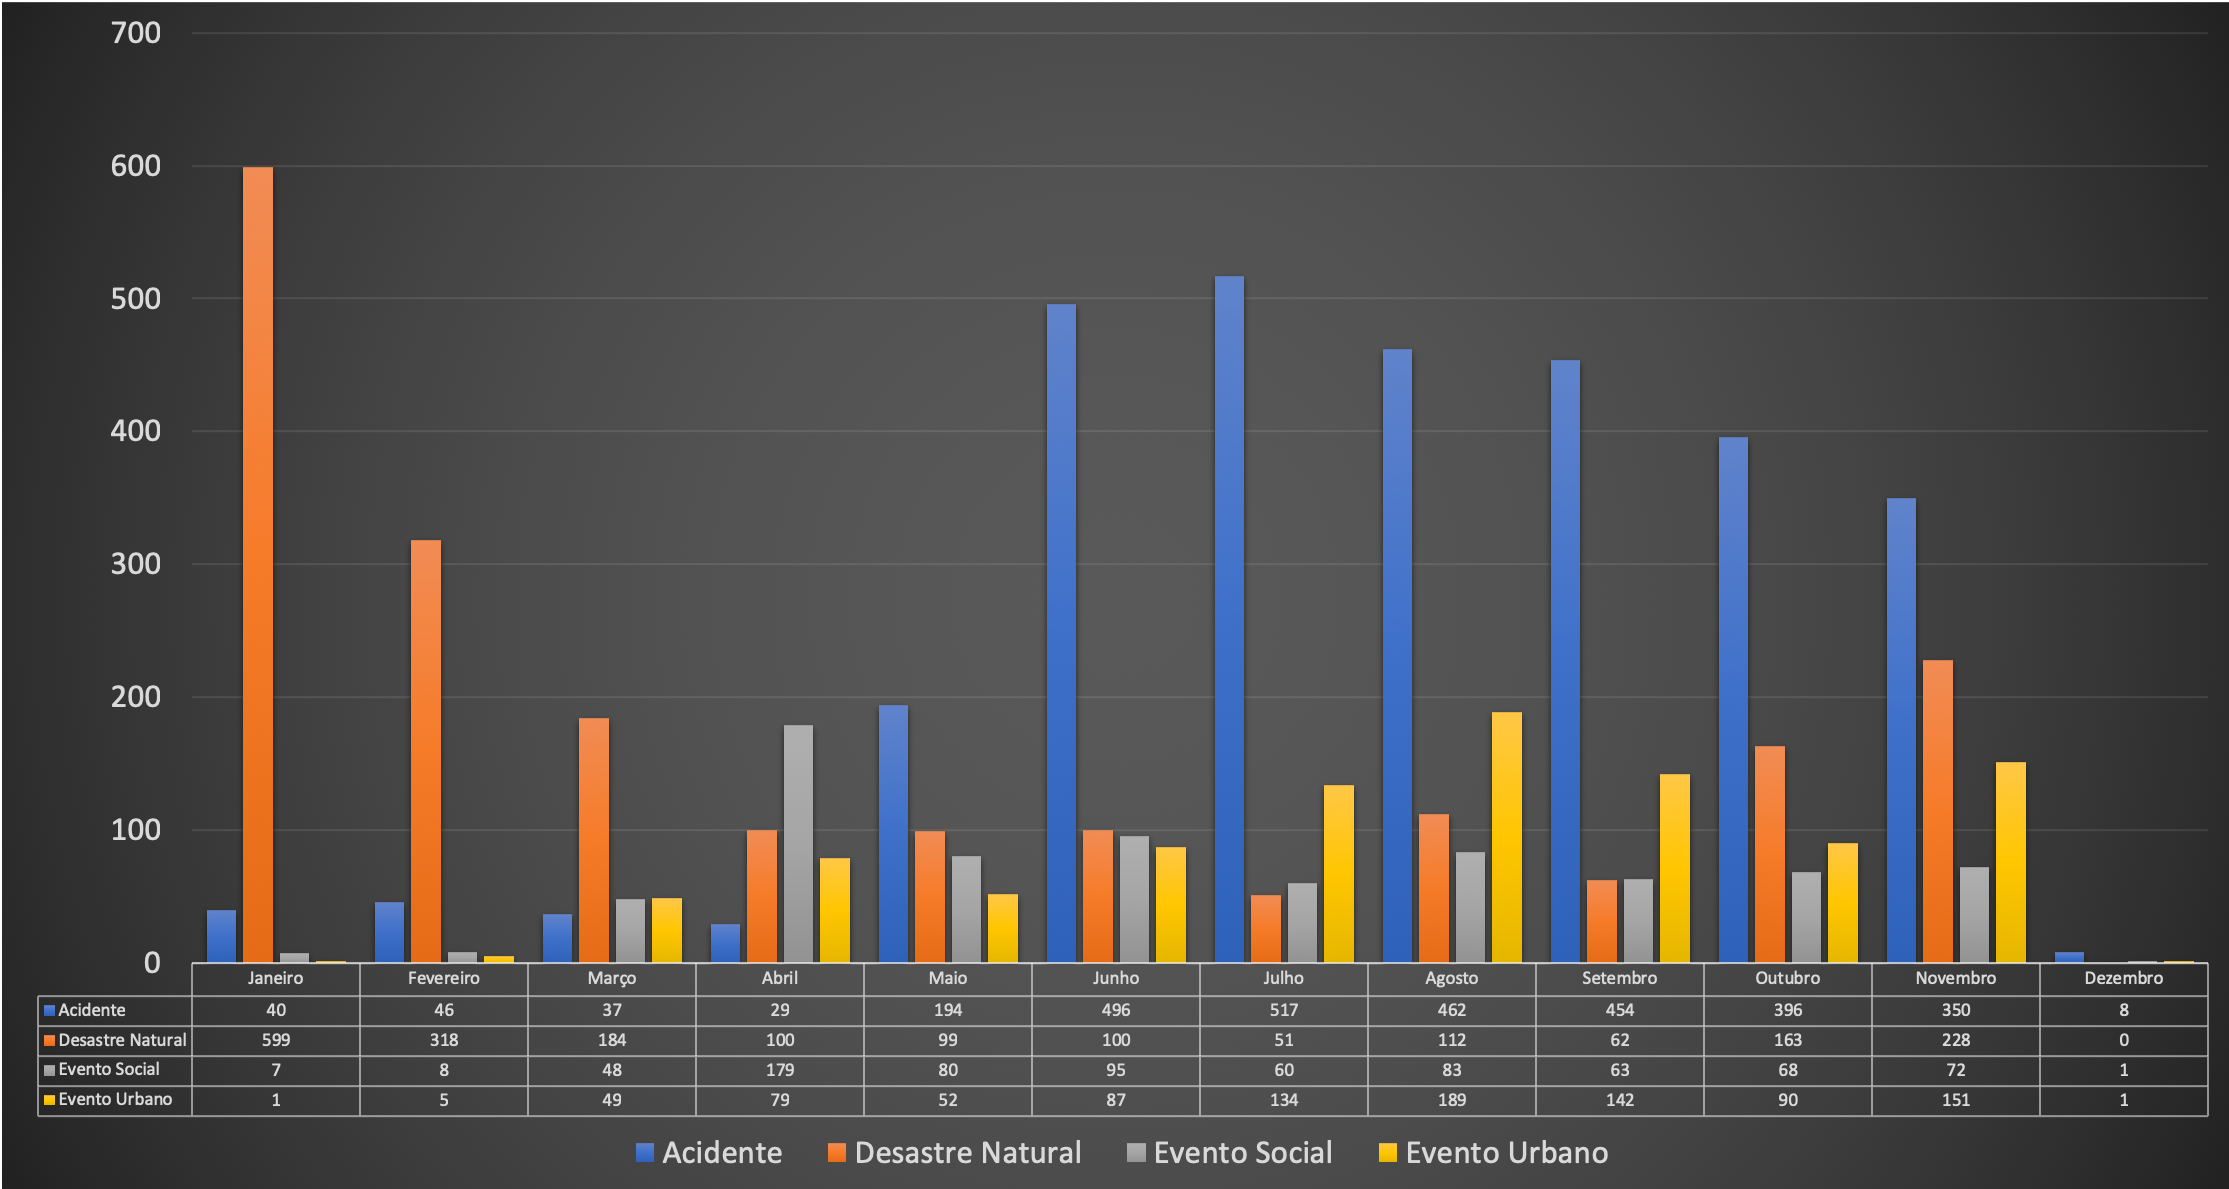
\includegraphics[width=0.8\linewidth]{exception_events_classification_distribution_pt.png}
	\label{fig:exception_events_classification_distribution}
\end{figure}
\end{frame}
%------------------------------------------------
\begin{frame}{Processo para correlação entre os dados AVL, GTFS e \textit{tweets} para análise do impacto dos eventos de exceção}
\begin{figure}[!htb]
	\centering
 	  \caption{Processo para correlação entre os dados AVL, GTFS e \textit{tweets} para análise do impacto dos eventos de exceção}
		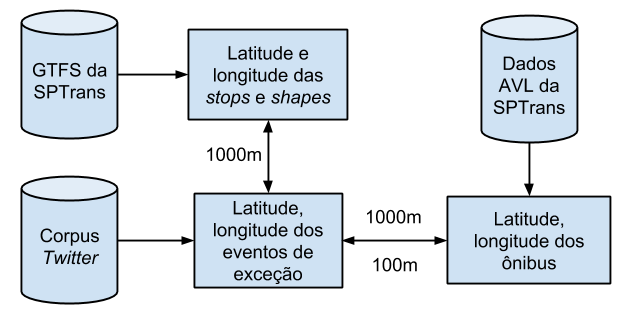
\includegraphics[width=1\linewidth]{avl_tweets_correlation_pt.png}
	\label{fig:avl_tweets_correlation_pt}
\end{figure} 
\end{frame}
%------------------------------------------------
\begin{frame}{Equação utilizada para identificar velocidade mediana esperada}
    \begin{equation}
\label{eqVeloc}
 f(n) =
  \begin{cases}
    0      & \quad \text{se  vel.~mediana~do~dia~do~evento} > \frac{\text{vel.~mediana~dos~dias~da~semana}}{\text{total~de~vel.~medianas}}\\
    1 & \quad \text{se vel.~mediana~do~dia~do~evento} \leq \frac{\text{vel.~mediana~dos~dias~da~semana}}{\text{total~de~vel.~medianas}}
  \end{cases}
\end{equation}
\end{frame}
%------------------------------------------------
\begin{frame}{Resultados da caracterização dos impactos em relação às velocidades medianas dos ônibus}
\begin{table}[!htb]
\centering
\caption {Porcentagem de ônibus dos grupos de linhas afetadas por eventos de exceção, a 1.000~m e 100~m de distância a partir dos pontos de parada, respectivamente, que tiveram a velocidade mediana reduzida nos meses do ano de 2017}
\label{tab:exceptEventVelocityImpAllStop}
\begin{adjustbox}{max height=10mm, width=3.5in}
\begin{tabular}{c|cc|cc|cc|cc}
\toprule
\textbf{Mês} & \multicolumn{2}{c}{\textbf{Acidente}} & \multicolumn{2}{c}{\textbf{Desastre Natural}} & \multicolumn{2}{c}{\textbf{Evento Social}} &
\multicolumn{2}{c}{\textbf{Evento Urbano}}\\
\cmidrule(l){2-3} \cmidrule(l){4-5} \cmidrule(l){6-7} \cmidrule(l){8-9}
 & 1.000 m & 100 m & 1.000 m & 100 m & 1.000 m & 100 m & 1.000 m & 100 m \\
\midrule
Janeiro & 83,33 &  100 & 
64,23 &  98,00 & 
100 & --- &
 100 & --- \\
\hline
Fevereiro & 70,58 &  100 &
 66,25 &  100 &
 100 & 100 &
 80 & --- \\
\hline
Março &  50,00 &  --- & 
66,66 &  100 &
85,00 & 100 &
68,18 & 100 \\
\hline
Abril & 87,50 &100 & 
 61,11 & 100 & 
 82,75 & 100 & 
 76,92 &  100 \\
\hline
Maio & 65,13 &  100 &
 58,82 &  100 &
 93,33 & 100 &
 50,00 & 100 \\
\hline
Junho & 54,46 &  100 &
 61,53 &  100 &
 76,47 & 100 &
 72,41 & 100 \\
\hline
Julho & 61,48 &  98,41 &
 66,66 & 100 &
 69,23 & 100 &
58,13 & 100 \\
\hline
Agosto & 57,86 & 87,17 &
 55,35 & 100 &
 85,54 & 100 & 
 68,10 & 90,90 \\
\hline
Setembro & 64,21 & 100 &
 42,10 & 100 &
 92,30 & 100 & 
 62,06 & 100 \\
\hline
Outubro & 70,49 & --- &
 56,81 & --- &
 80,00 & --- &
 61,11 & --- \\
\hline
Novembro & 66,66 & 100 &
 57,99 & 100 &
 92,85 & 100 &
 74,35 & 100 \\
\hline
Dezembro & --- & --- & --- & --- & --- & --- & --- & ---  \\
\midrule
\midrule
\textbf{Total} & 66,51 & 98,39 & 59,77 & 99,80 & 87,04 & 100 & 70,11 & 98,86  \\
\bottomrule
\end{tabular}
\end{adjustbox}
\end{table}
\end{frame}
%------------------------------------------------
\begin{frame}{Resultados da caracterização dos impactos em relação às velocidades medianas dos ônibus}
\begin{table}[!htb]
\centering
\caption {Porcentagem de impacto na velocidade média dos grupos de linhas afetadas por eventos de exceção a 1.000~m e 100~m de distância dos pontos de rota, respectivamente, nos meses do ano de 2017}
\label{tab:exceptEventVelocityImpAllShapes}
\begin{adjustbox}{max height=10mm, width=3.5in}
\begin{tabular}{c|cc|cc|cc|cc}
\toprule
\newline \textbf{Mês} & \multicolumn{2}{c}{\textbf{Acidente}} &
\multicolumn{2}{c}{\textbf{Desastre Natural}} & \multicolumn{2}{c}{\textbf{Evento Social}} &
\multicolumn{2}{c}{\textbf{Evento Urbano}}\\
\cmidrule(l){2-3} \cmidrule(l){4-5} \cmidrule(l){6-7} \cmidrule(l){8-9}
 & 1.000 m & 100 m & 1.000 m & 100 m & 1.000 m & 100 m & 1.000 m & 100 m \\
\midrule
Janeiro & 66,66 &  100 & 
 47,68 &  78,49 & 
 100 & 100 &
 100 & --- \\
\hline
Fevereiro & 35,29  &  100 &
 49,09 &  81,25 &
 100 & 100 &
 40,00 & 100 \\
\hline
Março  & 66,66  &  100 & 
 42,85 &  62,5 &
90,00 & 72,22 &
50,00 & 53,84 \\
\hline
Abril & 62,50 & 60,00 & 
47,05  & 100 & 
76,11 & 77,27 & 
89,47 &  90,90\\
\hline
Maio & 49,09 &  77,77 &
64,70 &  100 &
73,33 & 80,00 &
40,00 & 50,00 \\
\hline
Junho & 47,78 &  79,76 &
 46,15 &  70,00 &
 61,76 & 61,29 &
72,41 & 77,77 \\
\hline
Julho & 44,85  &  75,55 &
 66,66  & 83,33 &
48,14  & 75,00 &
41,86 & 61,53 \\
\hline
Agosto & 49,49 & 75,36 &
  44,44 & 71,42 &
  72,72 & 72,72 & 
70,00  & 56,75 \\
\hline
Setembro & 49,47  & 79,16 &
36,84  & 54,54 &
76,92  & 58,33 & 
55,17 & 73,91 \\
\hline
Outubro & 56,06 & 78,26 &
58,69  & 90,00 &
90,00  & 75,00 &
55,00 & 60,00 \\
\hline
Novembro & 54,32 & 66,66 &
 44,00 & 74,07 &
85,71  & 85,71 &
67,50  & 72,97 \\
\hline
Dezembro & --- & --- & --- & --- & --- & --- & --- & ---  \\
\midrule
\midrule
\textbf{Total} & 52,92 & 81,13 & 49,83 & 78,69 & 79,51 & 77,95 & 68,14 & 69,76  \\
\bottomrule
\end{tabular}
\end{adjustbox}
\end{table}
\end{frame}
%------------------------------------------------
\begin{frame}{Trabalhos relacionados a identificação de padrões de velocidade média dos dados AVL}
\begin{itemize}
    \item Algoritmo Apriori e a análise de cluster para encontrar padrões relacionados a transferência (entre metrô e ônibus), por meio dos dados dos cartões inteligentes usados no transporte público da China.
    \item Algoritmo Apriori utilizado para identificar os padrões existentes nos conjuntos de dados relacionados a movimentação diária no transporte público de Singapura e no MIT Reality Mining Data. O sistema desenvolvido é capaz de identificar e apresentar visualmente padrões de movimentação humana, em relação ao espaço e ao tempo. 
    \item Algoritmo Apriori utilizado para identificar padrões de rotas de táxi, na cidade de Pequim, China.
    \item Algoritmo Apriori utilizado para identificar e classificar as anomalias no comportamento do trânsito, por meio de agregações espaço-temporais usando o algoritmo Apriori, aplicadas aos dados de transporte rodoviário da cidade do Rio de Janeiro.
\end{itemize}
\end{frame}
%------------------------------------------------
\begin{frame}{Identificação de padrões de velocidade média dos dados AVL}
\begin{block}{}
        A proposta desse experimento se diferencia das demais por encontrar os padrões de velocidade média existentes nos dados do transporte público por ônibus da cidade de São Paulo, considerando ainda a correlação com eventos de exceção extraídos de Redes Sociais.
\end{block}
\end{frame}
%------------------------------------------------
\begin{frame}{Resultados da identificação de padrões de velocidade média dos dados AVL}
\begin{table}[!htb]
\centering
\caption {Análise \textit{Apriori}\tnote{a} aplicada as velocidades médias (intervalos de 5 minutos) ao conjunto de dados AVL da SPTrans}
\label {tab:aprioriFull}
\begin{adjustbox}{max height=10mm, width=4in}
\begin{tabular}{c|c|c|c|c}
\toprule
\textbf{Mês} & \textbf{Regra de associação} & \textit{\textbf{Support}} & \textit{\textbf{Confidence}} & \textit{\textbf{Lift}} \\
\midrule
Fevereiro & 7 $\rightarrow$ 8 & 0,101 & 0,496 & 3,586\\
Abril & 7 $\rightarrow$ 8  & 0,108 & 0,456 & 3,188\\
Maio & 7 $\rightarrow$ 8 & 0,108 & 0,570 & 4,375\\
\midrule
Outubro & 8 $\rightarrow$ 7 & 0,100 & 0,595 & 3,433\\
Novembro & 8 $\rightarrow$ 7 & 0,104 & 0,446 & 3,369\\
\midrule
Janeiro & 11 $\rightarrow$ 12 & 0,137 & 0,476 & 1,729 \\
Junho & 11 $\rightarrow$ 12 & 0,129 & 0,632 & 1,656\\
Julho & 11 $\rightarrow$ 12 & 0,204 & 0,694 & 1,934\\
Agosto & 11 $\rightarrow$ 12 & 0,169 & 0,670 & 1,662\\
Outubro & 11 $\rightarrow$ 12 & 0,119 & 0,601 & 1,669\\
\bottomrule
\end{tabular}
\end{adjustbox}
\end{table}
\end{frame}
%------------------------------------------------
\begin{frame}{Resultados da identificação de padrões de velocidade média dos dados AVL}
\begin{table}[!htb]
\centering
\caption {(Continuação) Análise \textit{Apriori}\tnote{a} aplicada as velocidades médias (intervalos de 5 minutos) ao conjunto de dados AVL da SPTrans}
\label {tab:aprioriFull}
\begin{adjustbox}{max height=10mm, width=4in}
\begin{tabular}{c|c|c|c|c}
\toprule
\textbf{Mês} & \textbf{Regra de associação} & \textit{\textbf{Support}} & \textit{\textbf{Confidence}} & \textit{\textbf{Lift}} \\
\midrule
Fevereiro & 12 $\rightarrow$ 11 & 0,126 & 0,582 & 1,770\\
Março & 12 $\rightarrow$ 11 & 0,134 & 0,621 & 1,627\\
Abril & 12 $\rightarrow$ 11 & 0,123 & 0,601 & 2,013\\
Maio & 12 $\rightarrow$ 11 & 0,137 & 0,645 & 1,703\\
Setembro & 12 $\rightarrow$ 11 & 0,163 & 0,608 & 1,863\\
Novembro & 12 $\rightarrow$ 11 & 0,154 & 0,531 & 1,875\\
Dezembro & 12 $\rightarrow$ 11 & 0,143 & 0,432 & 2,073\\
\midrule
Fevereiro & 12 $\rightarrow$ 13 & 0,123 & 0,375 & 1,956\\
Março & 12 $\rightarrow$ 13 & 0,158 & 0,415 & 1,766\\
Junho & 12 $\rightarrow$ 13 & 0,141 & 0,370 & 1,907\\
\bottomrule
\end{tabular}
\end{adjustbox}
\end{table}
\end{frame}
%------------------------------------------------
\begin{frame}{Resultados da identificação de padrões de velocidade média dos dados AVL}
\begin{table}[!htb]
\centering
\caption {(Fim da continuação) Análise \textit{Apriori}\tnote{a} aplicada as velocidades médias (intervalos de 5 minutos) ao conjunto de dados AVL da SPTrans}
\label {tab:aprioriFull}
\begin{adjustbox}{max height=10mm, width=4in}
\begin{tabular}{c|c|c|c|c}
\toprule
\textbf{Mês} & \textbf{Regra de associação} & \textit{\textbf{Support}} & \textit{\textbf{Confidence}} & \textit{\textbf{Lift}} \\
\midrule
Abril  & 13 $\rightarrow$ 12 & 0,109 & 0,367 & 2,280\\
Maio & 13 $\rightarrow$ 12 & 0,161 & 0,425 & 1,942\\
Agosto & 13 $\rightarrow$ 12 & 0,147 & 0,366 & 1,830\\
Outubro & 13 $\rightarrow$ 12 & 0,150 & 0,417 & 1,737\\
\bottomrule
\end{tabular}
\end{adjustbox}
\end{table}
\end{frame}
%------------------------------------------------
\begin{frame}{Resultados das velocidades médias inesperadas correlacionadas aos eventos de exceção (ref. aos pontos de parada)}
\begin{figure}[!htb]
	\centering
 	  \caption{Velocidades inesperadas dos ônibus impactados por eventos de exceção relacionados a acidentes a 100~m e 1.000~m dos pontos de parada, ao longo dos meses do ano de 2017}
		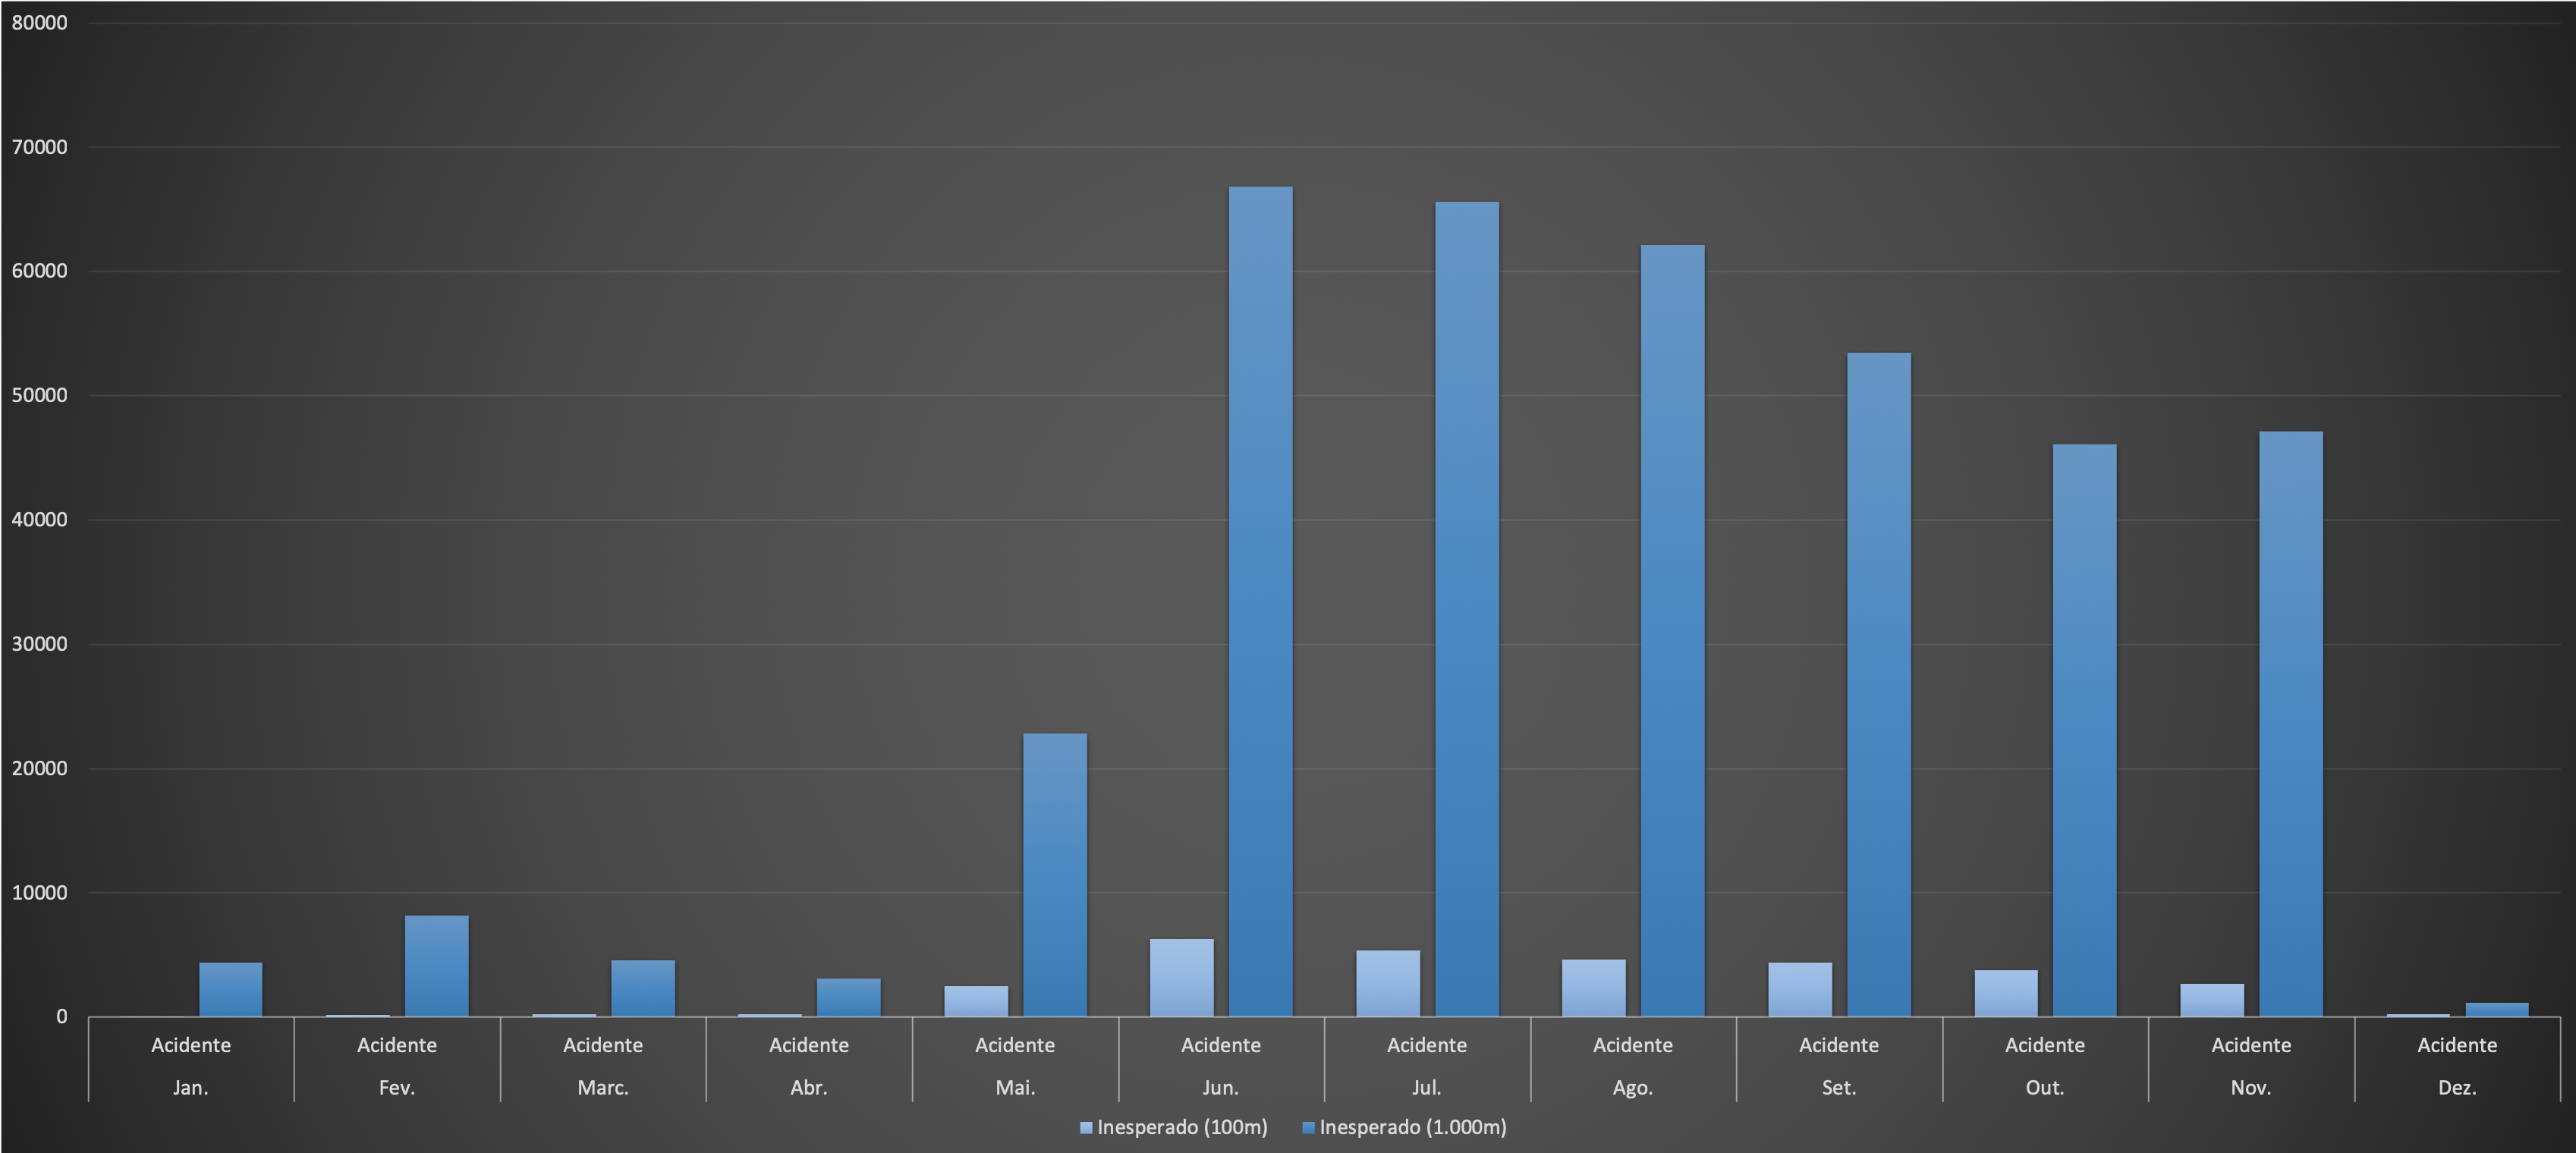
\includegraphics[width=0.8\linewidth]{apriori_analysis_stops_accidents.png}
	\label{fig:apriori_analysis_stops_accidents}
\end{figure}
\end{frame}
%------------------------------------------------
\begin{frame}{Resultados das velocidades médias inesperadas correlacionadas aos eventos de exceção (ref. aos pontos de parada)}
\begin{figure}[!htb]
	\centering
 	  \caption{Velocidades inesperadas dos ônibus impactados por eventos de exceção relacionados a desastres naturais a 100~m e 1.000~m dos pontos de parada, ao longo dos meses do ano de 2017}
		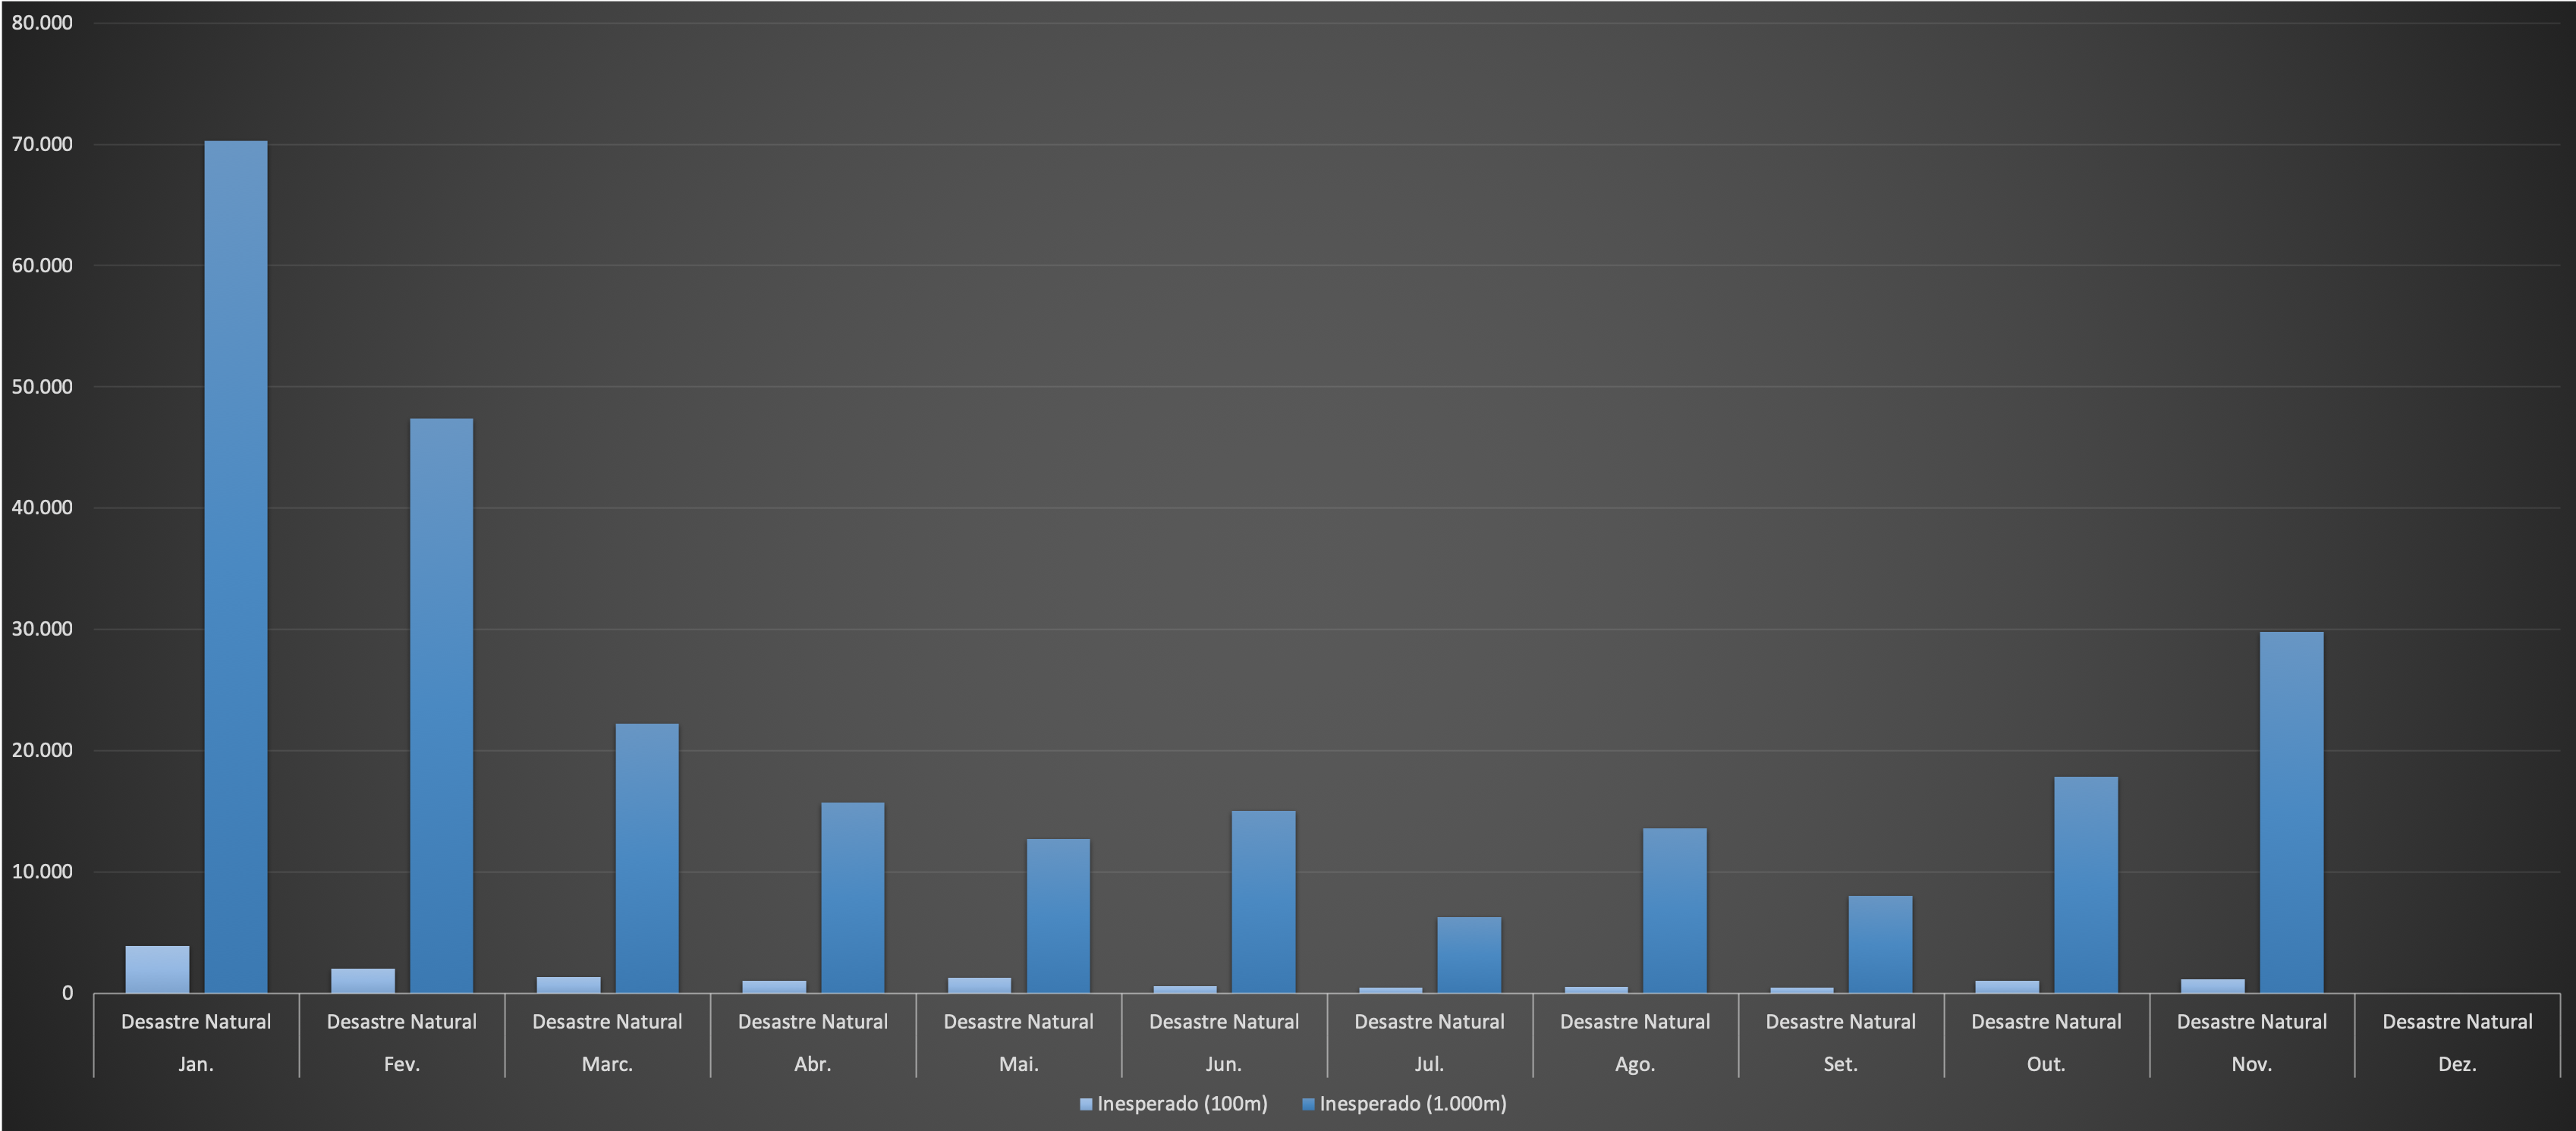
\includegraphics[width=0.8\linewidth]{apriori_analysis_stops_natural_disasters.png}
	\label{fig:apriori_analysis_stops_natural_disasters}
\end{figure}
\end{frame}
%------------------------------------------------
\begin{frame}{Resultados das velocidades médias inesperadas correlacionadas aos eventos de exceção (ref. aos pontos de parada)}
\begin{figure}[!htb]
	\centering
 	  \caption{Velocidades inesperadas dos ônibus impactados por eventos de exceção relacionados a eventos sociais a 100~m e 1.000~m dos pontos de parada, ao longo dos meses do ano de 2017}
		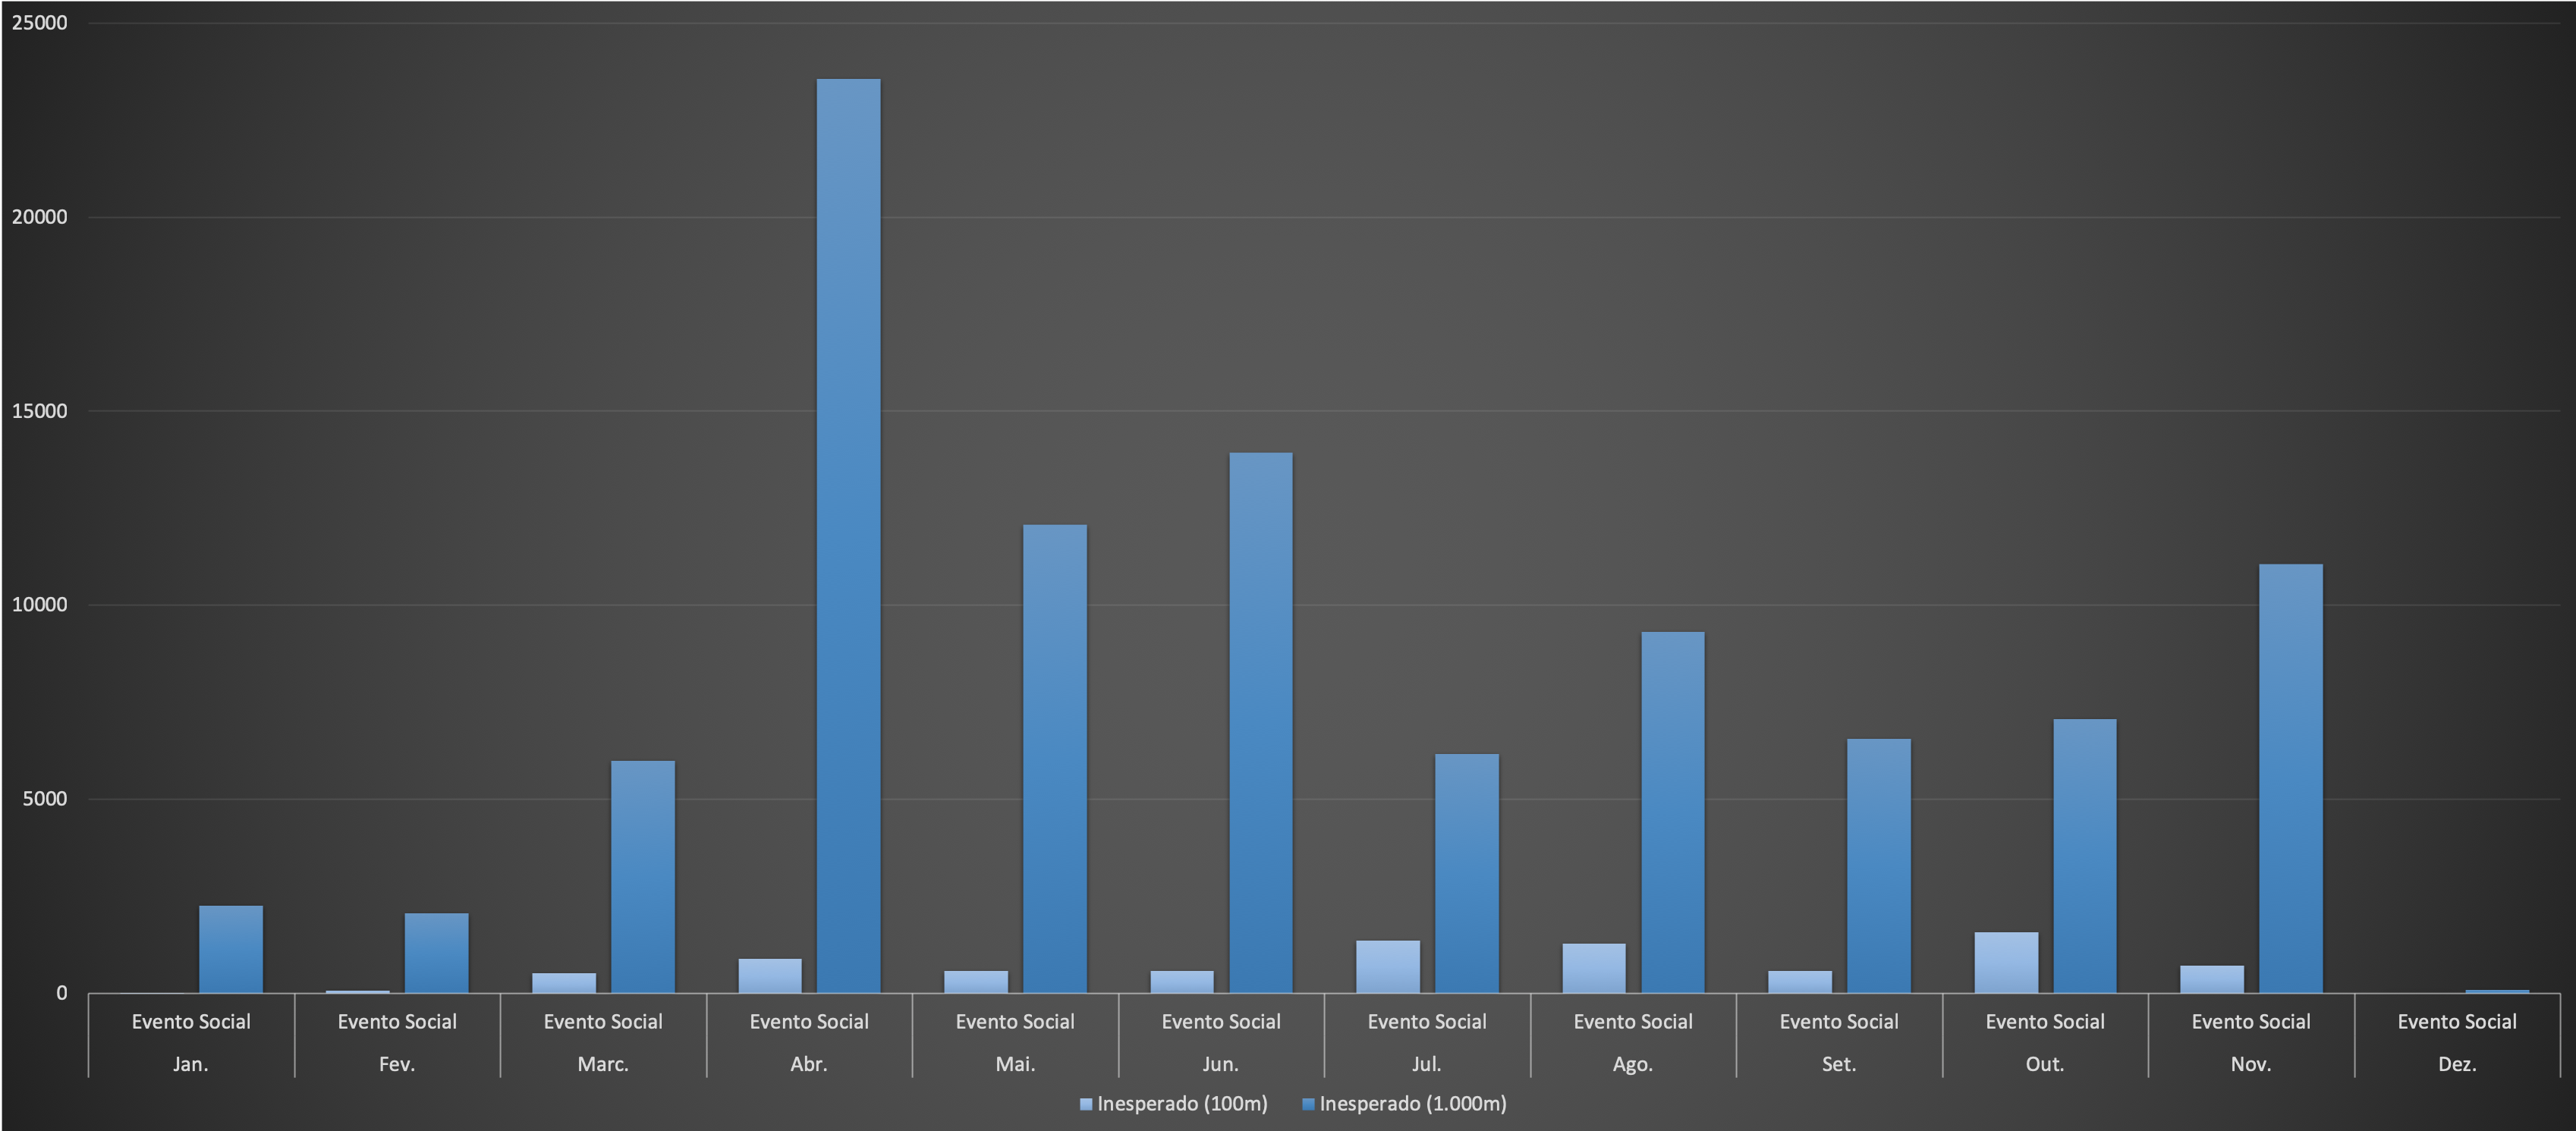
\includegraphics[width=0.8\linewidth]{apriori_analysis_stops_social_events.png}
	\label{fig:apriori_analysis_stops_social_events}
\end{figure}
\end{frame}
%------------------------------------------------
\begin{frame}{Resultados das velocidades médias inesperadas correlacionadas aos eventos de exceção (ref. aos pontos de parada)}
\begin{figure}[!htb]
	\centering
 	  \caption{Velocidades inesperadas dos ônibus impactados por eventos de exceção relacionados a eventos urbanos a 100~m e 1.000~m dos pontos de parada, ao longo dos meses do ano de 2017}
		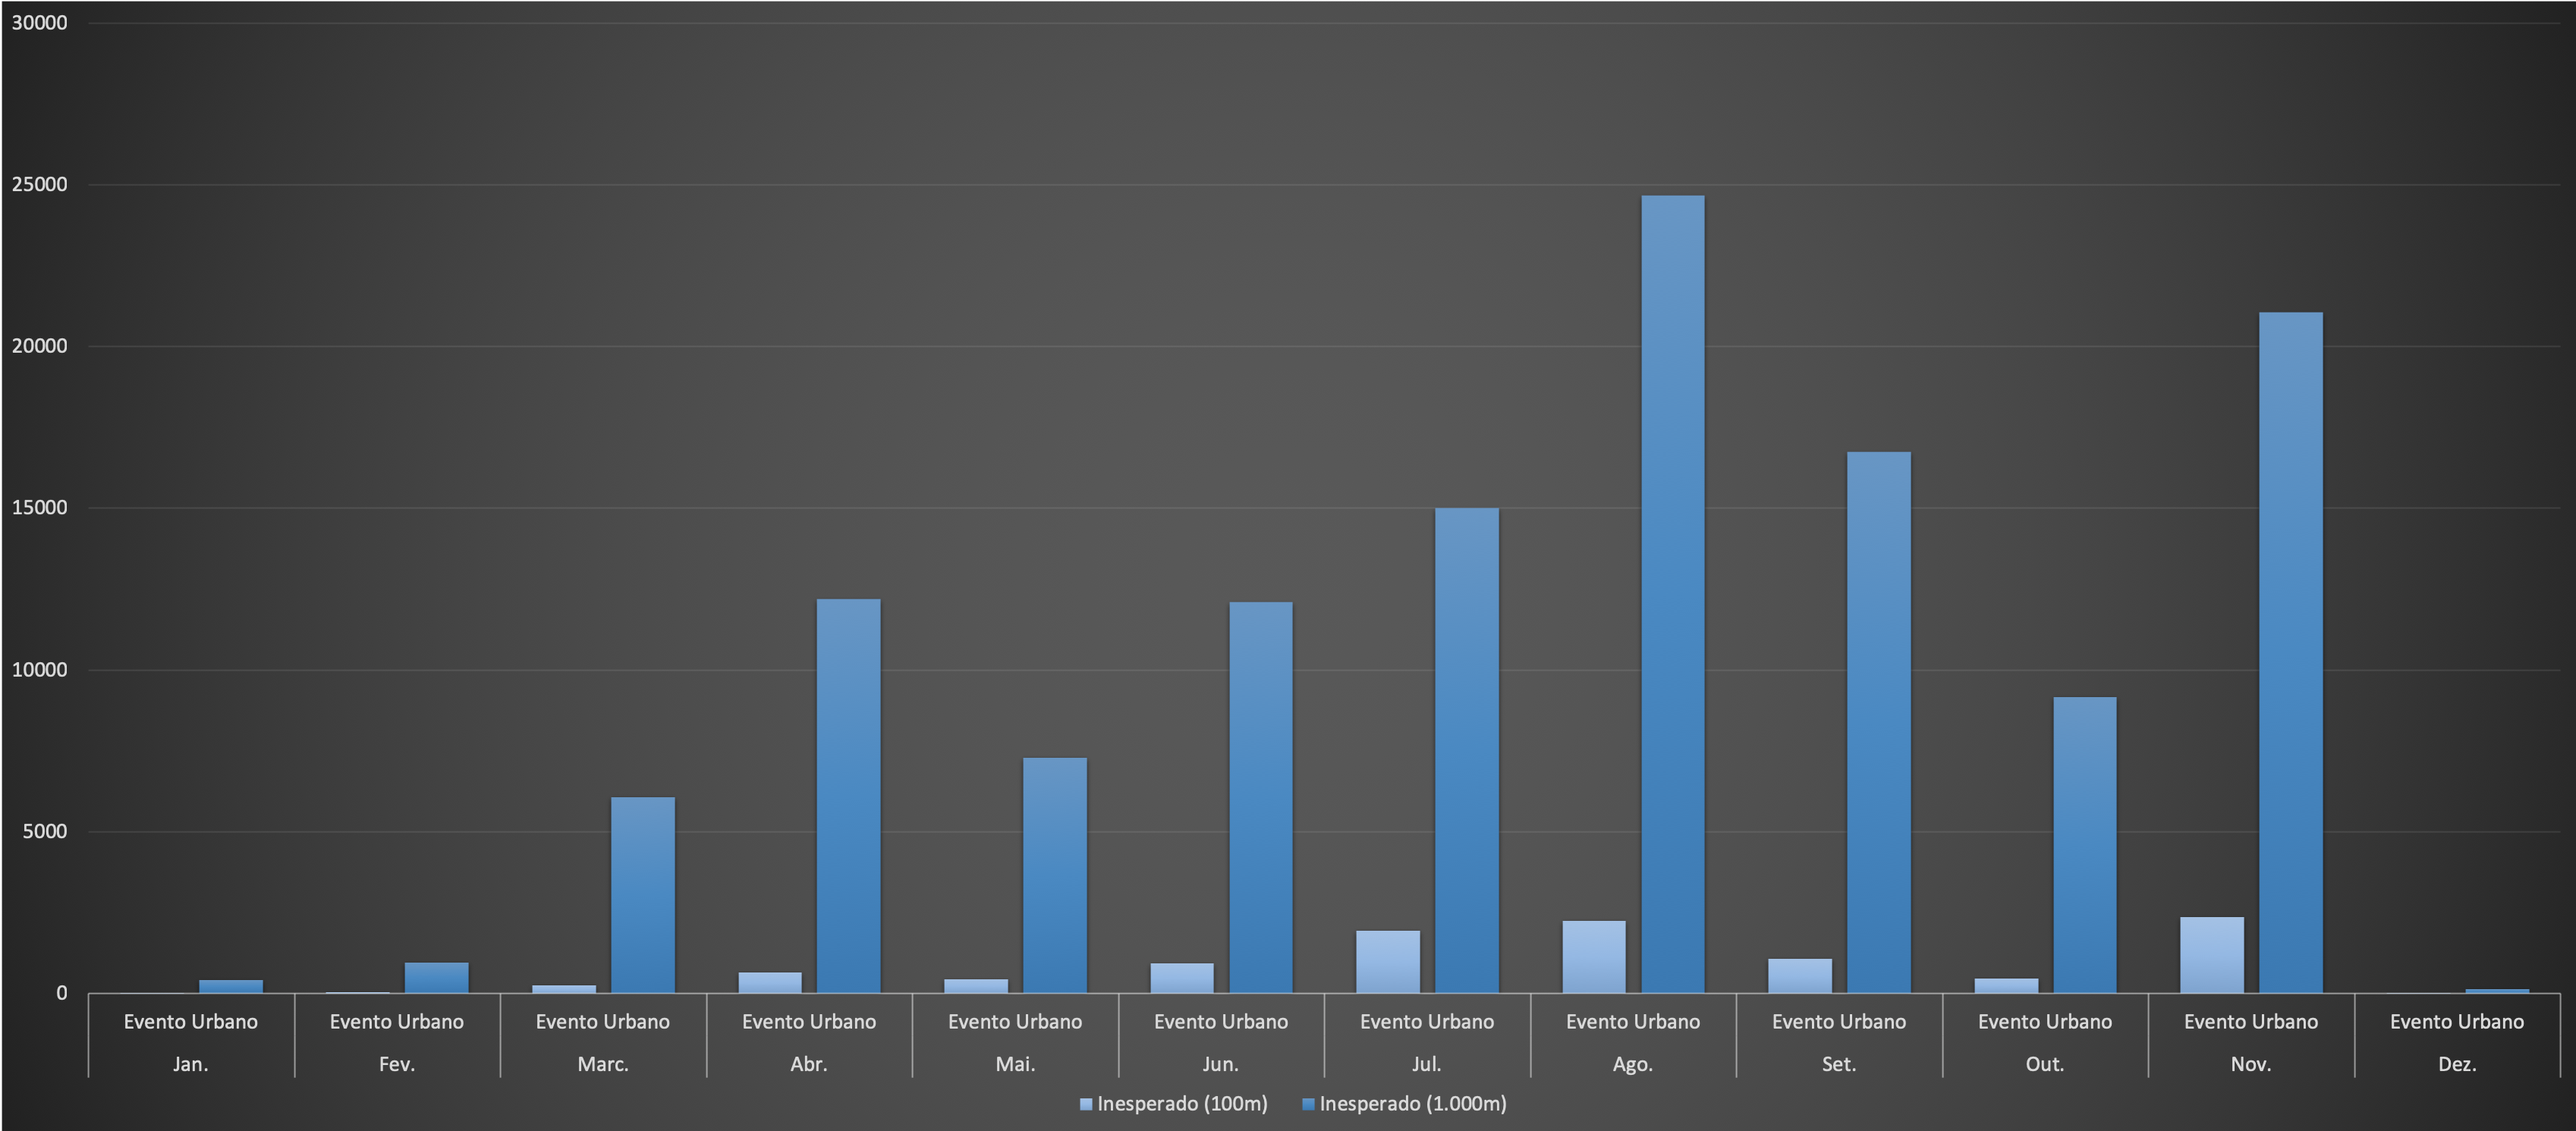
\includegraphics[width=0.8\linewidth]{apriori_analysis_stops_urban_events.png}
	\label{fig:apriori_analysis_stops_urban_events}
\end{figure}
\end{frame}
%------------------------------------------------
\begin{frame}{Resultados das velocidades médias inesperadas correlacionadas aos eventos de exceção (ref. aos pontos de rota)}
    \begin{figure}[!htb]
	\centering
 	  \caption{Velocidades inesperadas dos ônibus impactados por eventos de exceção relacionados a acidentes a 100~m e 1.000~m dos pontos de rota, ao longo dos meses do ano de 2017}
		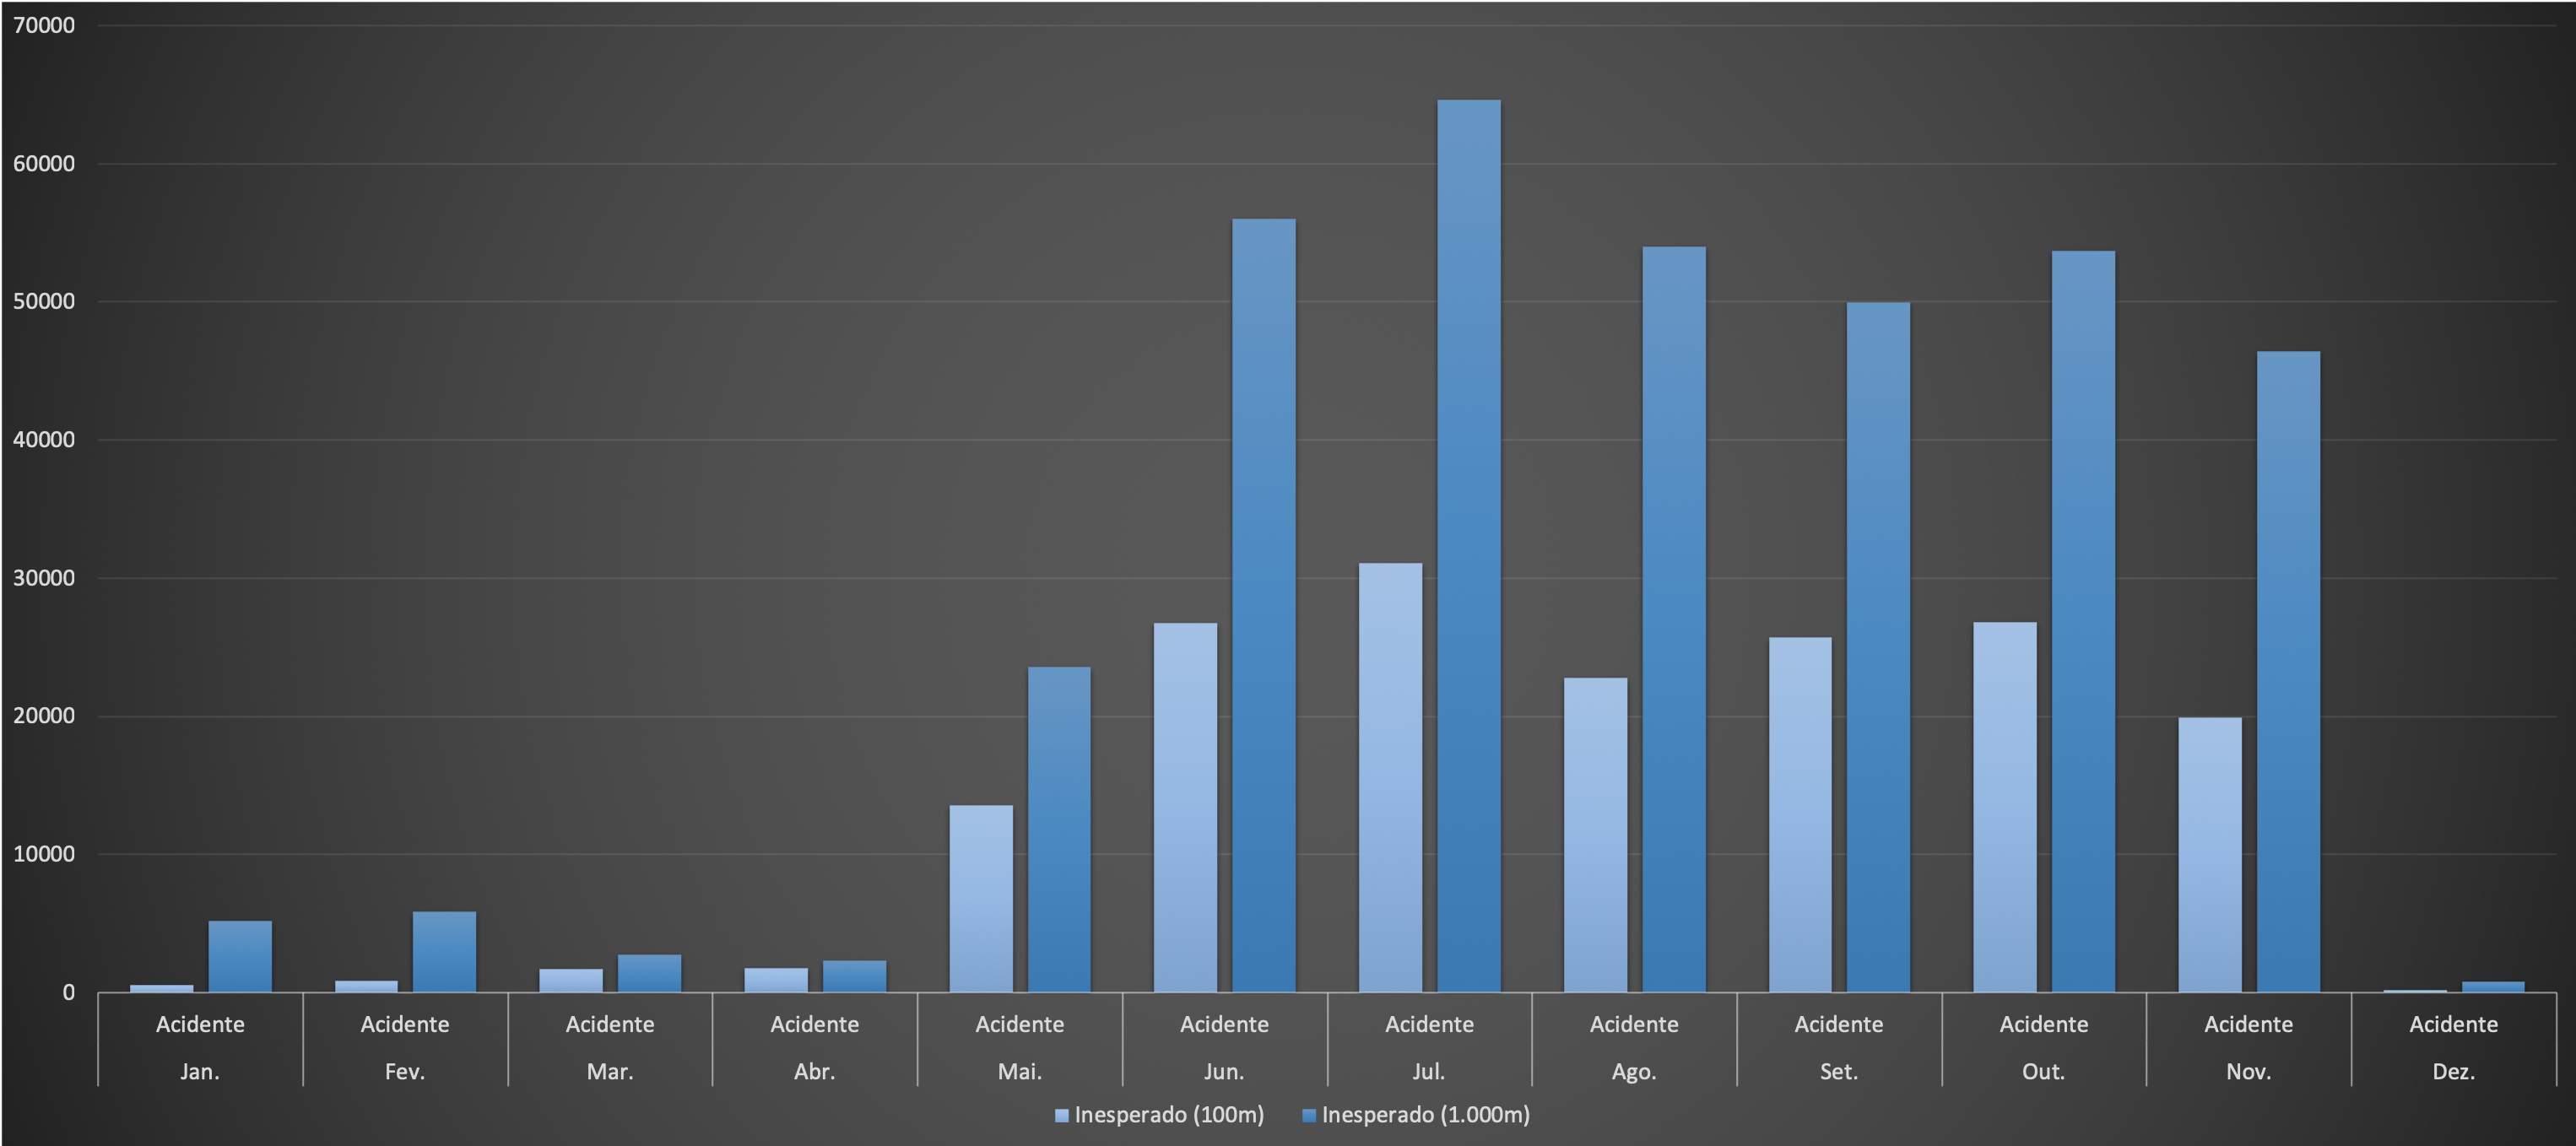
\includegraphics[width=0.8\linewidth]{apriori_analysis_shapes_accidents.png}
	\label{fig:apriori_analysis_shapes_accidents}
\end{figure}
\end{frame}
%------------------------------------------------
\begin{frame}{Resultados das velocidades médias inesperadas correlacionadas aos eventos de exceção (ref. aos pontos de rota)}
    \begin{figure}[!htb]
	\centering
 	  \caption{Velocidades inesperadas dos ônibus impactados por eventos de exceção relacionados a desastres naturais a 100~m e 1.000~m dos pontos de rota, ao longo dos meses do ano de 2017}
		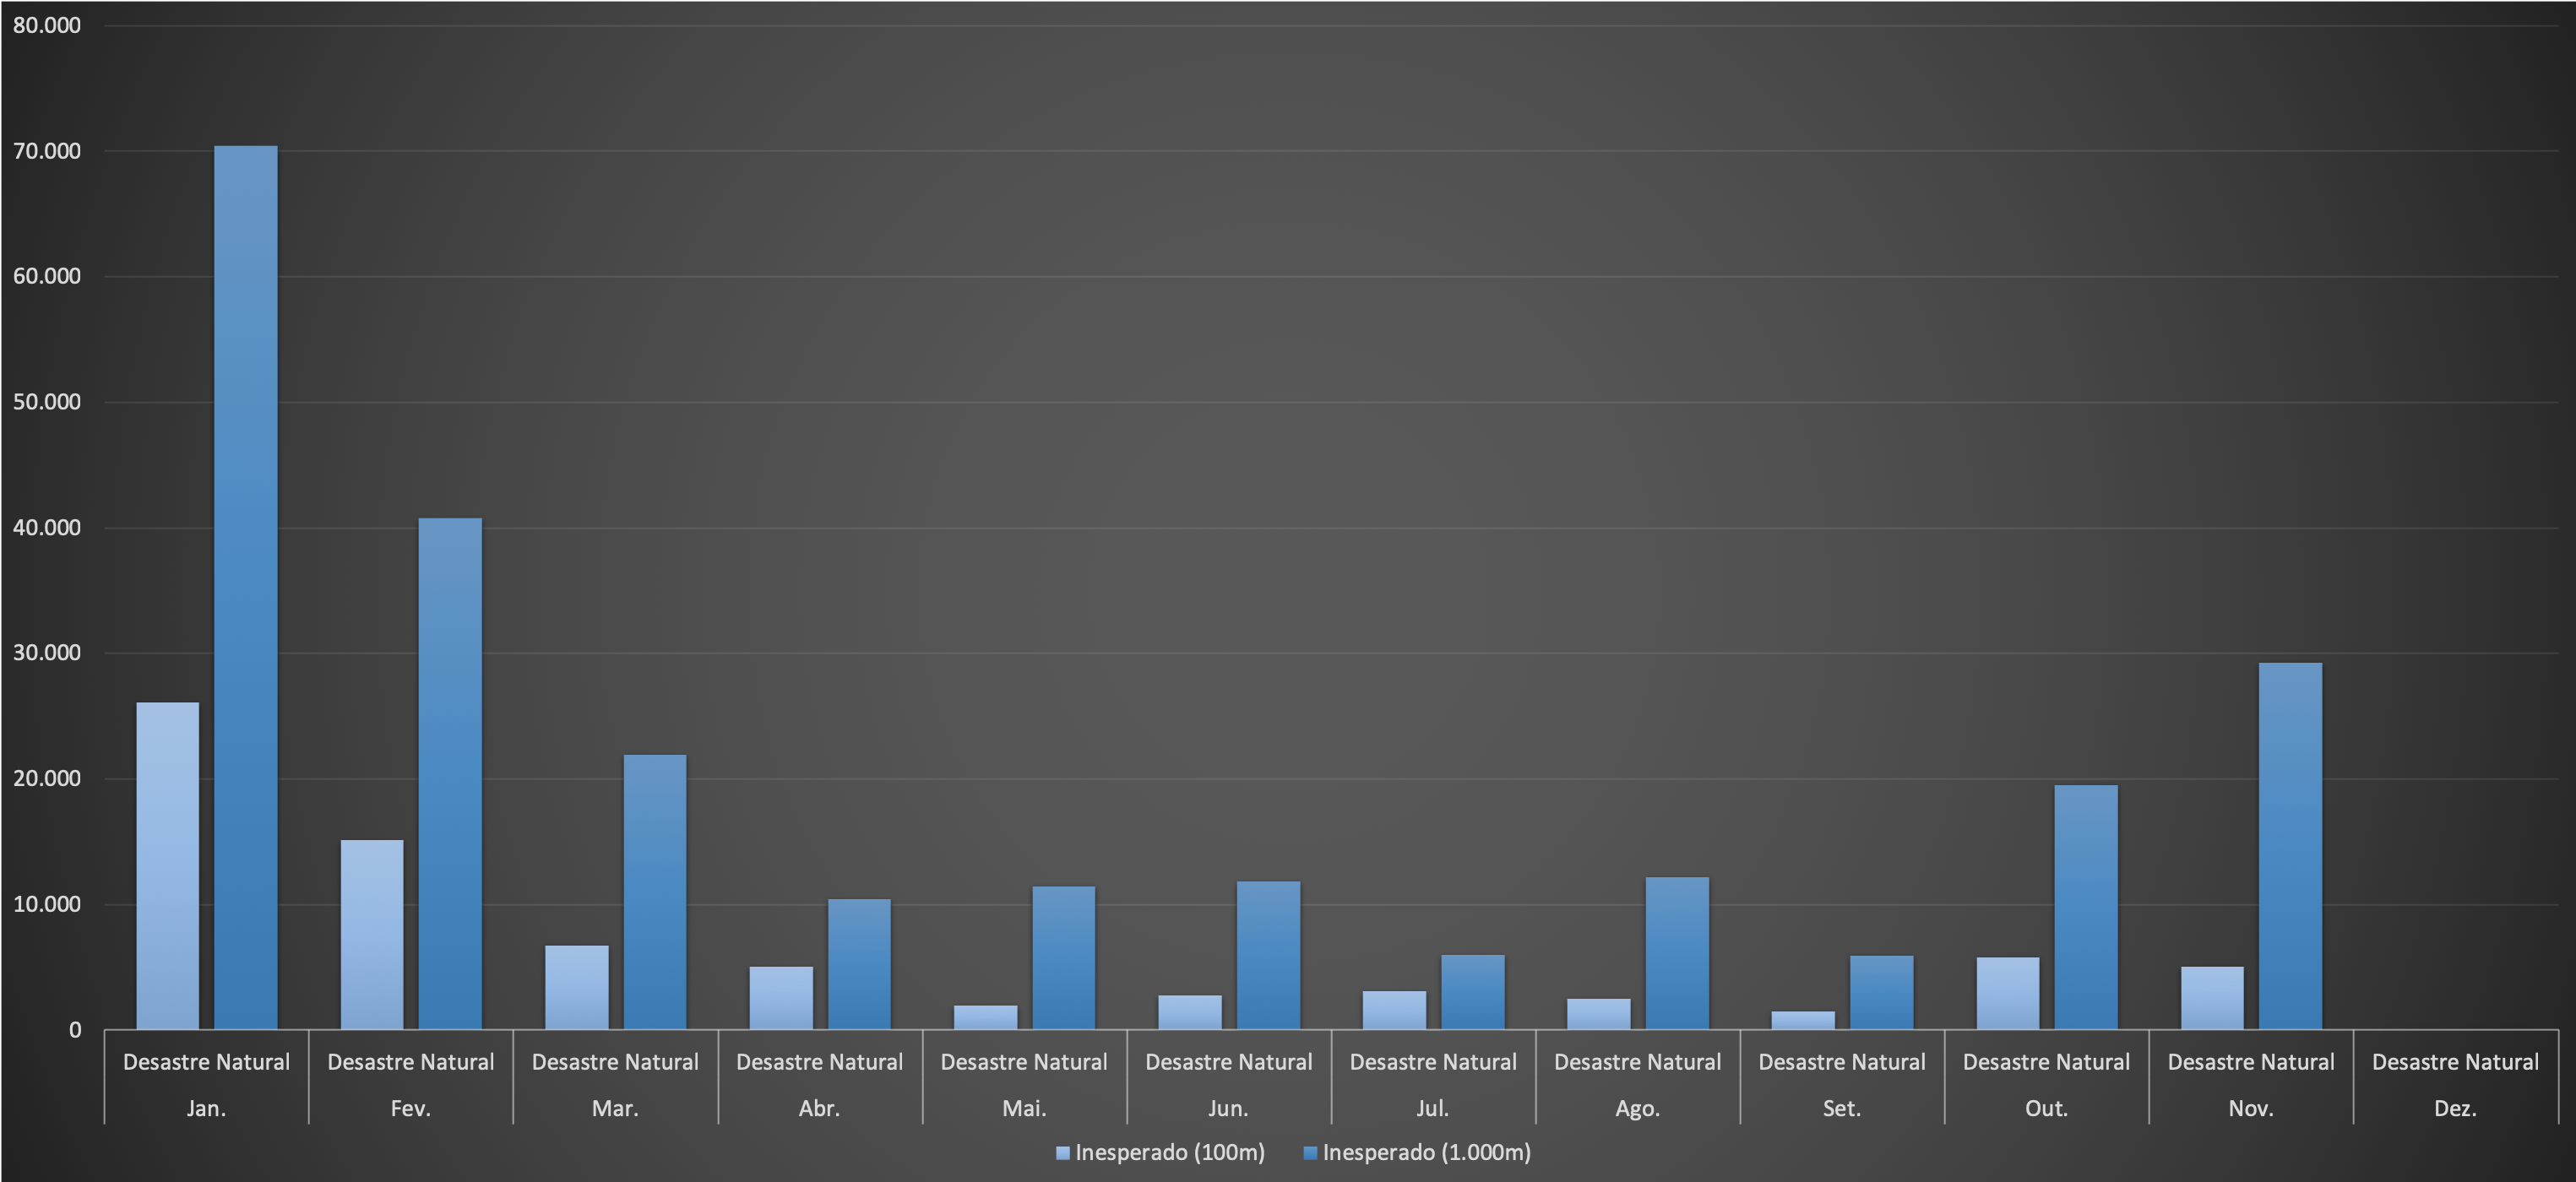
\includegraphics[width=0.8\linewidth]{apriori_analysis_shapes_natural_disasters.png}
	\label{fig:apriori_analysis_shapes_natural_disasters}
\end{figure}
\end{frame}
%------------------------------------------------
\begin{frame}{Resultados das velocidades médias inesperadas correlacionadas aos eventos de exceção (ref. aos pontos de rota)}
\begin{figure}[!htb]
	\centering
 	  \caption{Velocidades inesperadas dos ônibus impactados por eventos de exceção relacionados a eventos sociais a 100~m e 1.000~m dos pontos de rota, ao longo dos meses do ano de 2017}
		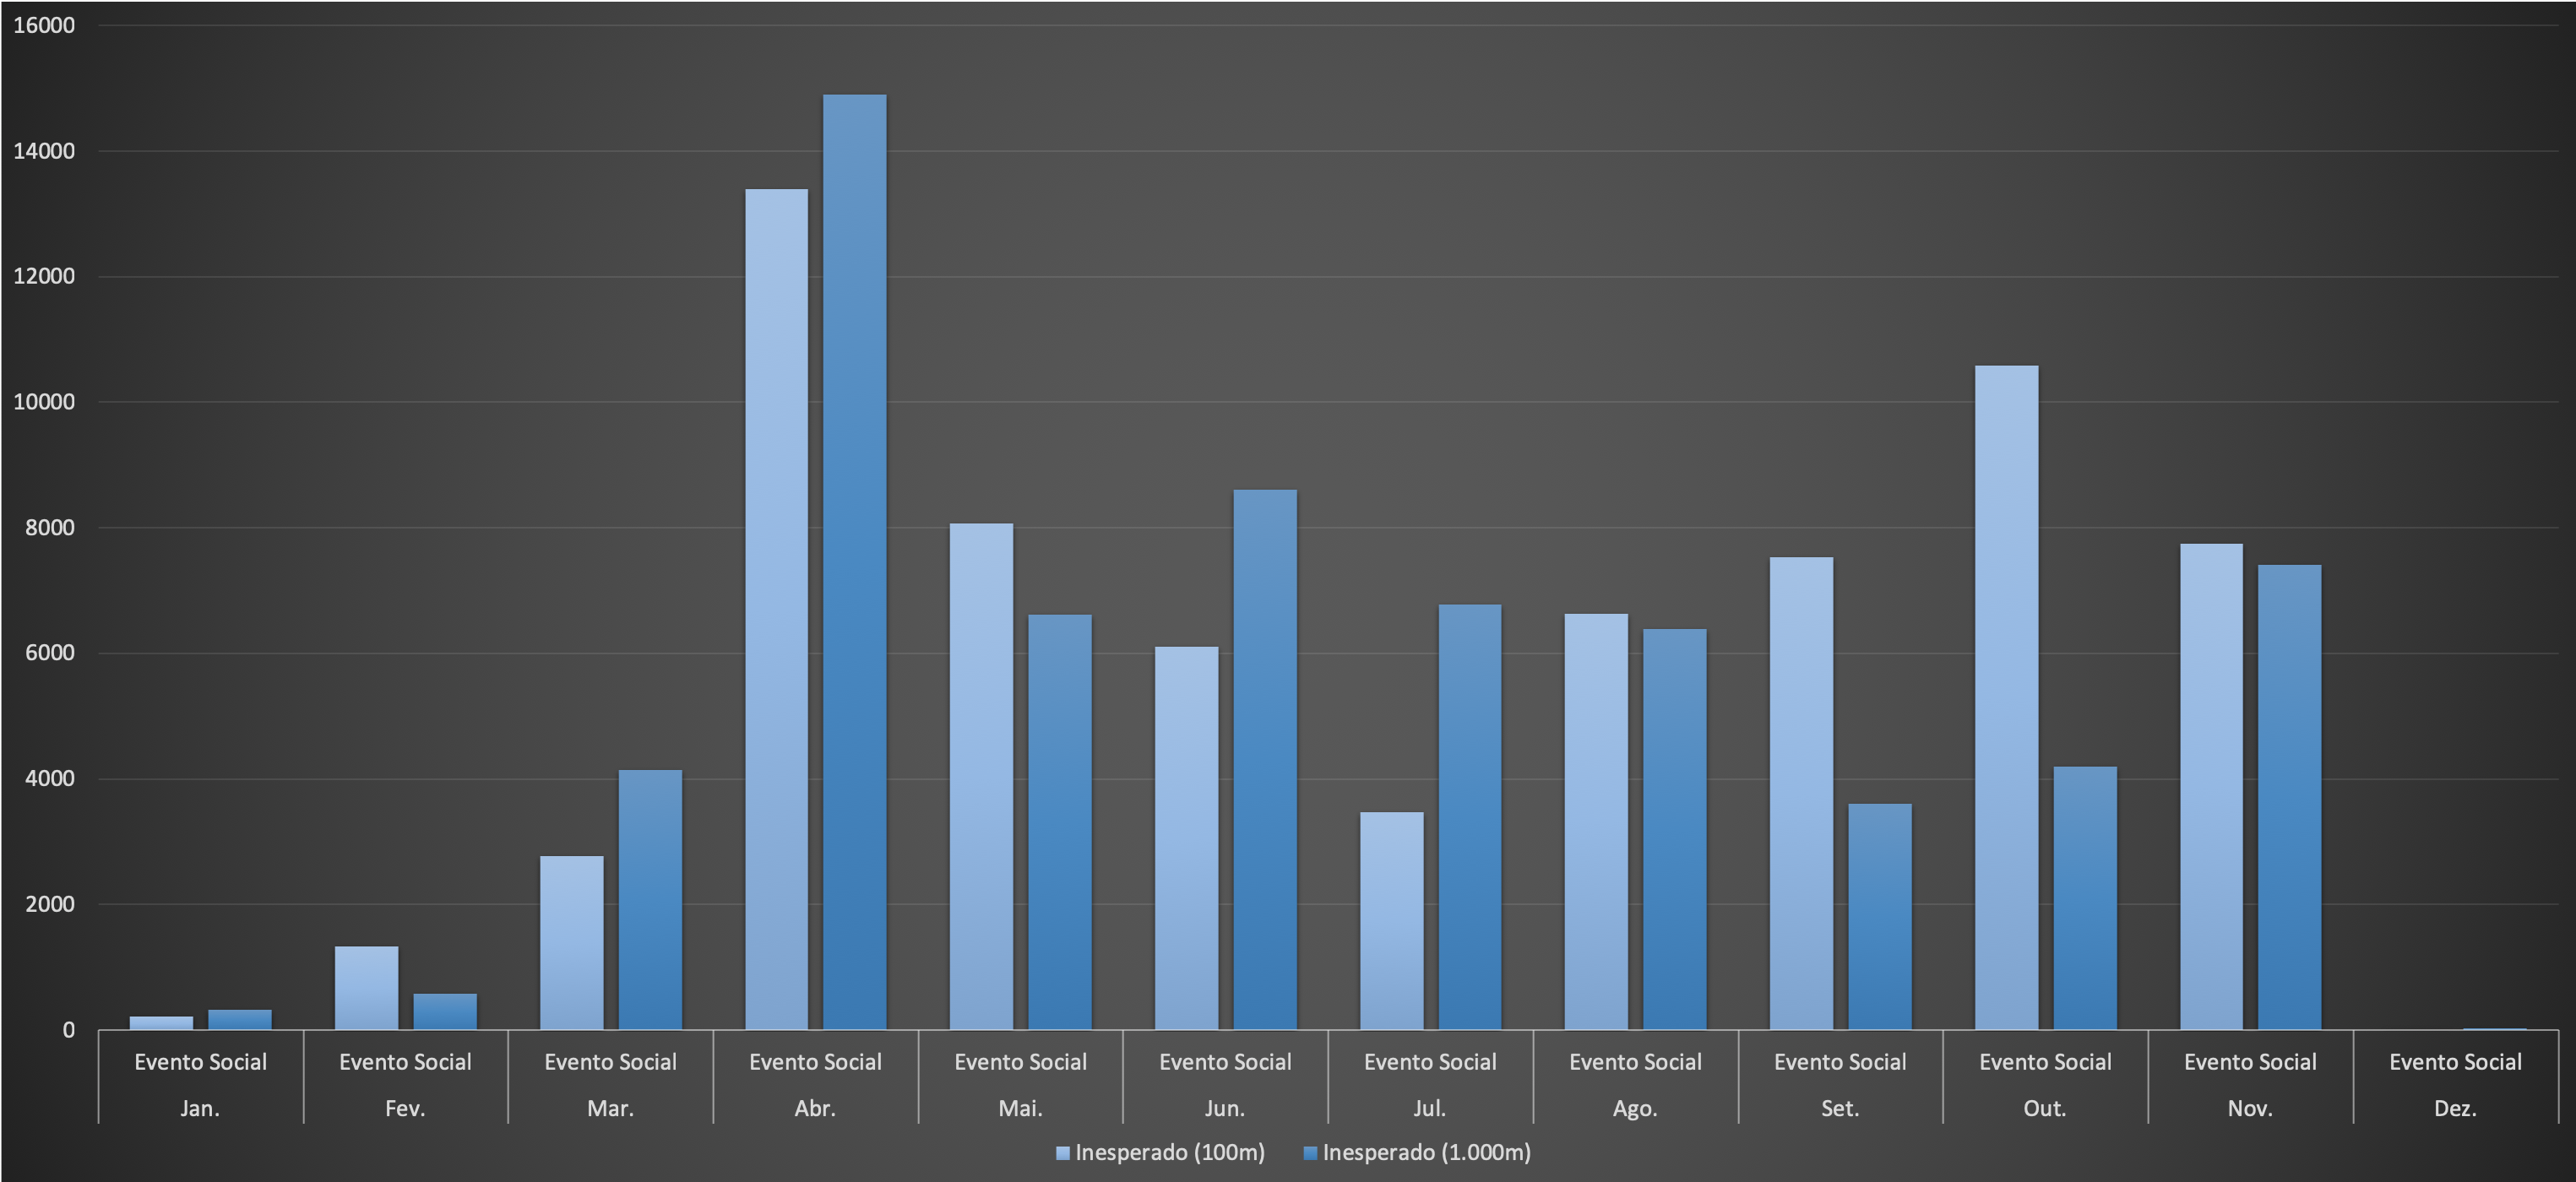
\includegraphics[width=0.8\linewidth]{apriori_analysis_shapes_social_events.png}
	\label{fig:apriori_analysis_shapes_social_events}
\end{figure}
\end{frame}
%------------------------------------------------
\begin{frame}{Resultados das velocidades médias inesperadas correlacionadas aos eventos de exceção (ref. aos pontos de rota)}
    \begin{figure}[!htb]
	\centering
 	  \caption{Velocidades inesperadas dos ônibus impactados por eventos de exceção relacionados a eventos sociais a 100~m e 1.000~m dos pontos de rota, ao longo dos meses do ano de 2017}
		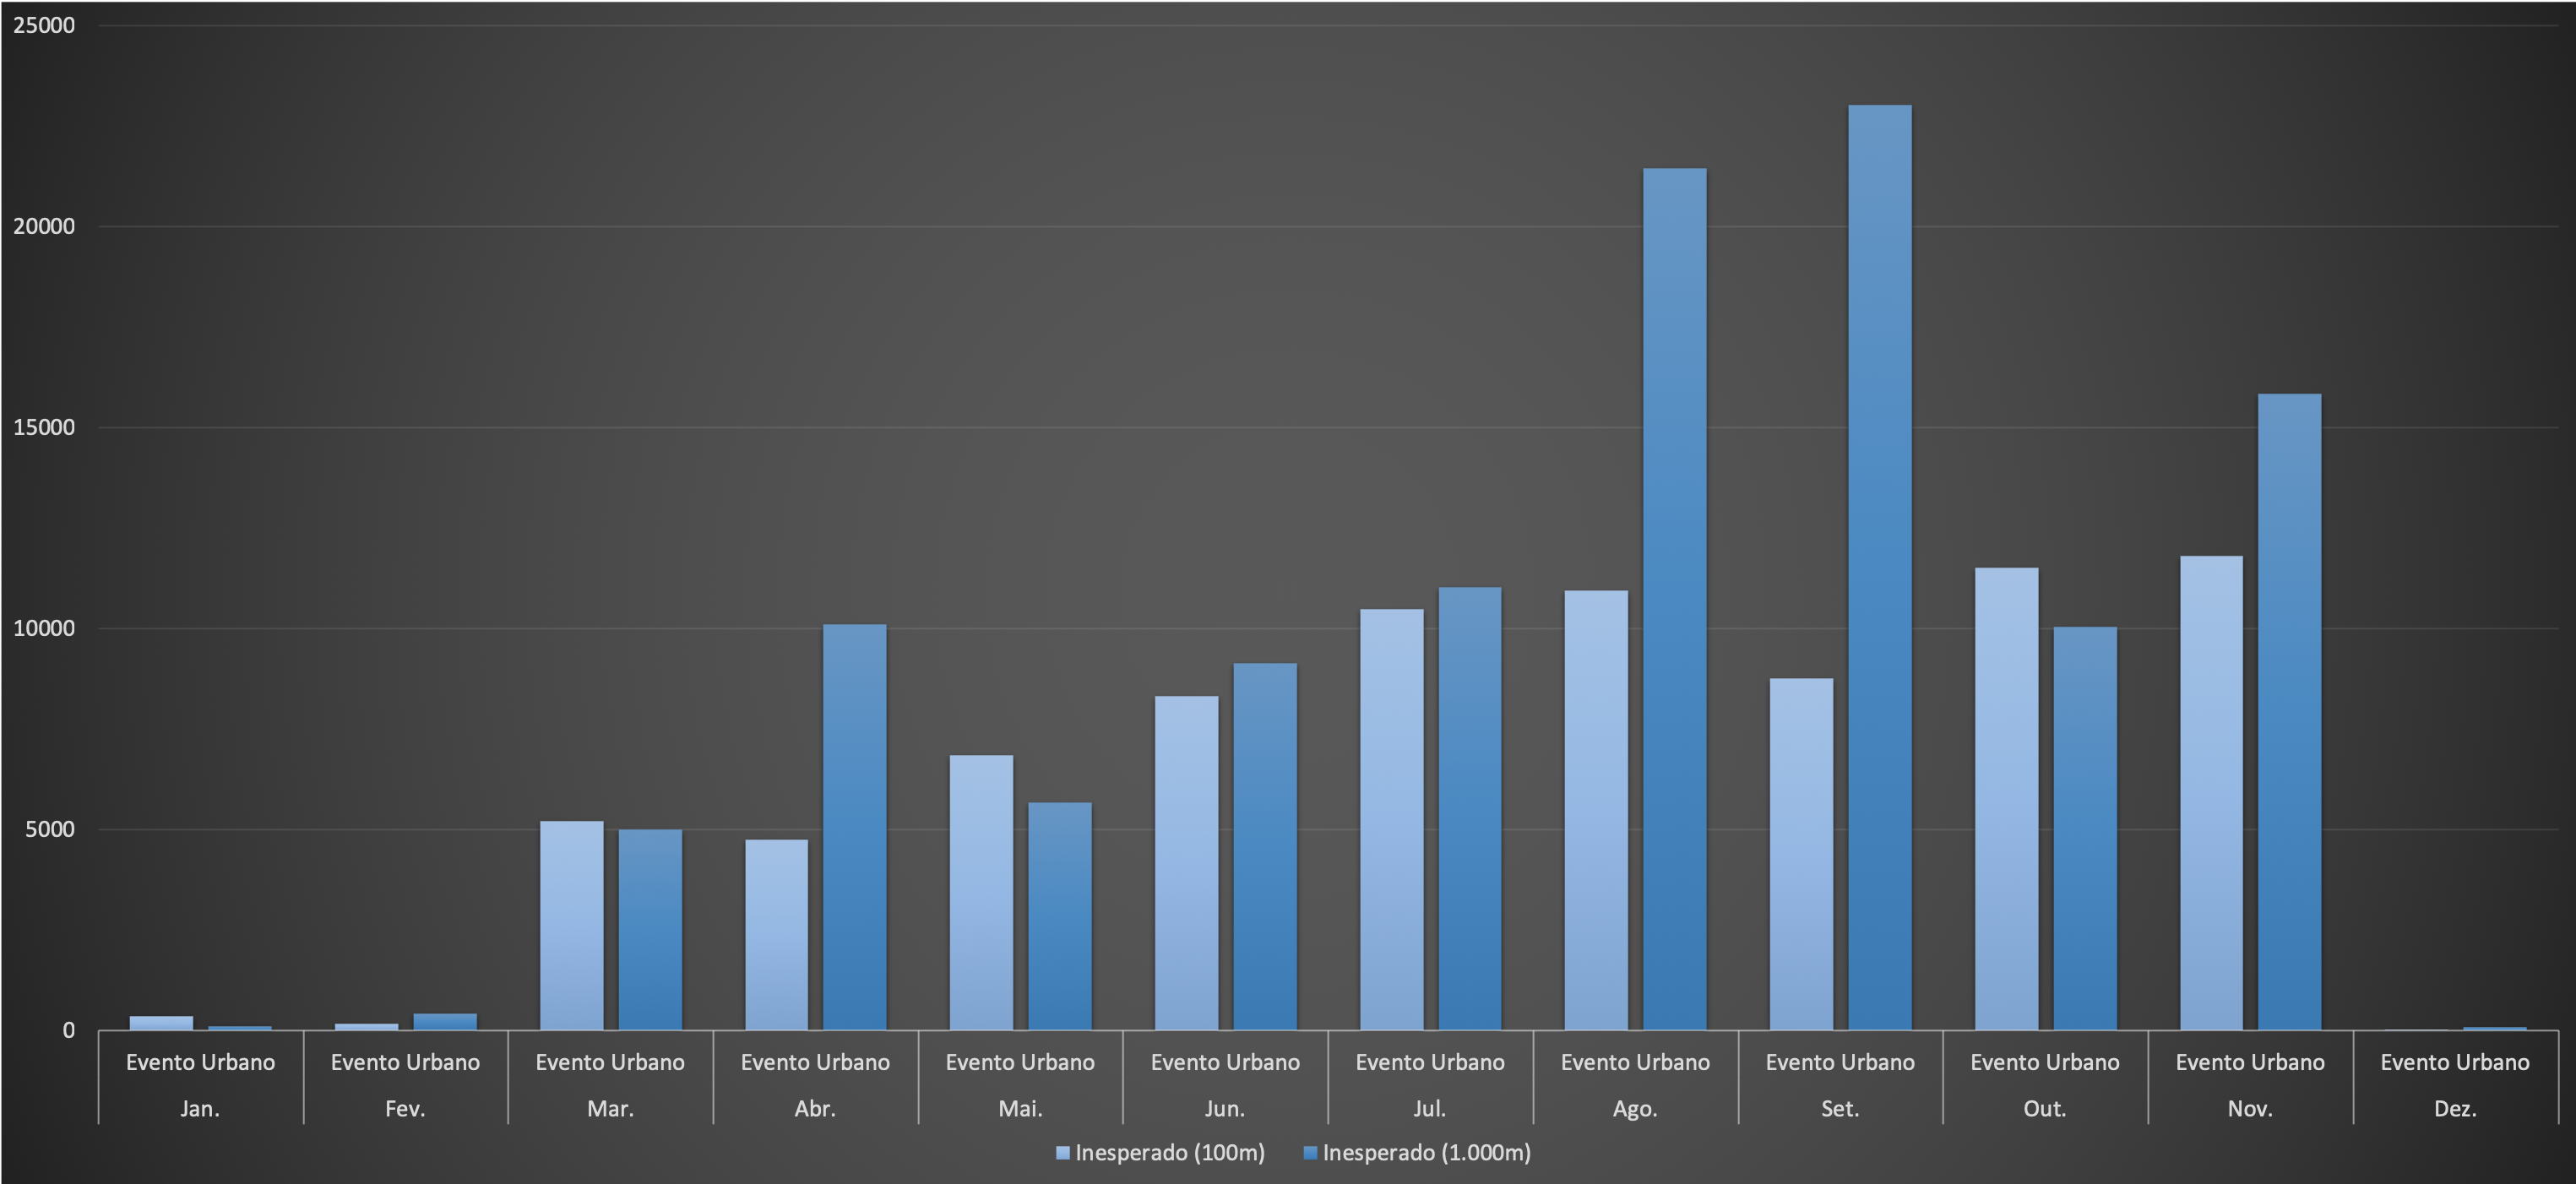
\includegraphics[width=0.8\linewidth]{apriori_analysis_shapes_urban_events.png}
	\label{fig:apriori_analysis_shapes_urban_events}
\end{figure}
\end{frame}
%------------------------------------------------
\begin{frame}
\begin{table}[!htb]
\centering
\begin{adjustbox}{max height=10mm, width=3in}
\begin{threeparttable}
\caption {Análise \textit{Apriori} aplicada as velocidades médias (intervalos de 5 minutos) ao conjunto de dados AVL da SPTrans correlacionados aos eventos de exceção (a distância de 100~m\tnote{f} e 1.000~m\tnote{g}, respectivamente, dos pontos de parada de ônibus) dos meses do ano de 2017}
\label {tab:aprioriExceptFullStops}
\begin{tabular}{c|c|c|c|c|c}
\toprule
\begin{tabular}{@{}c@{}}\textbf{Classe}\\ \textbf{do evento}\end{tabular} & \begin{tabular}{@{}c@{}}\textbf{Total de}\\ \textbf{eventos}\tnote{a}\end{tabular}  & \begin{tabular}{@{}c@{}}\textbf{Total de Regras }\\ \textbf{de Associação}\tnote{b}\end{tabular}  & \textbf{Esperadas}\tnote{c} & \begin{tabular}{@{}c@{}}\textbf{Não}\\ \textbf{esperadas}\tnote{d}\end{tabular}  & \begin{tabular}{@{}c@{}}\textbf{Parcialmente}\\ \textbf{inesperadas}\tnote{e}\end{tabular} \\
\midrule
Acidente & 1.677 & 315.063 & 278.493 & 30.804 & 5.766 \\
\hline
\begin{tabular}{@{}c@{}}Desastre\\ Natural\end{tabular} &  912 & 115.301 & 99.206 & 14.282 & 1.813 \\
\hline
\begin{tabular}{@{}c@{}}Evento\\ Social\end{tabular} & 506 & 61.927 & 52.403 & 8.245 & 1.279 \\
\hline
\begin{tabular}{@{}c@{}}Evento\\ Urbano\end{tabular}  & 596 & 93.513 & 81.261 & 10.480 & 1.772 \\
\midrule
\textbf{Total} & 3.691 & 585.804 & 511.363 & 63.811 & 10.603 \\
\bottomrule
\toprule
\begin{tabular}{@{}c@{}}\textbf{Classe}\\ \textbf{do evento}\end{tabular} & \begin{tabular}{@{}c@{}}\textbf{Total de}\\ \textbf{eventos}\tnote{a}\end{tabular}  & \begin{tabular}{@{}c@{}}\textbf{Total de Regras }\\ \textbf{de Associação}\tnote{b}\end{tabular}  & \textbf{Esperadas}\tnote{c} & \begin{tabular}{@{}c@{}}\textbf{Não}\\ \textbf{esperadas}\tnote{d}\end{tabular}  & \begin{tabular}{@{}c@{}}\textbf{Parcialmente}\\ \textbf{inesperadas}\tnote{e}\end{tabular} \\
\midrule
Acidente & 3.029 & 3.980.542 & 3.415.780 & 385.728 & 179.034 \\
\hline
\begin{tabular}{@{}c@{}}Desastre\\ Natural\end{tabular} &  2.016 & 2.624.415 & 2.253.123 & 259.285 & 112.007 \\
\hline
\begin{tabular}{@{}c@{}}Evento\\ Social\end{tabular} & 764 & 1.262.805 & 1.118.546 & 100.224 & 44.035 \\
\hline
\begin{tabular}{@{}c@{}}Evento\\ Urbano\end{tabular}  & 980 & 1.481.040 & 1.296.476 & 125.803 & 58.761 \\
\midrule
\textbf{Total} & 6.789 & 9.348.802 & 8.083.925 & 871.040 & 393.837 \\
\bottomrule
\end{tabular}
\begin{tablenotes}
            \item[a] Total de eventos de exceção.
            \item[b] Total de correlações de velocidade média.
            \item[c] Regras esperadas ($Lift > 1$, $Support > 0,05$)
            \item[d] Regras de associação inesperadas ($Lift = 1$).
            \item[e] Regras de associação parcialmente inesperadas ($0 < Lift < 1$).
            \item[f] 3.545 eventos de exceção não atingiram linhas de ônibus no raio de 100~m.
            \item[g] 447 eventos de exceção não atingiram linhas de ônibus no raio de 1.000~m.
        \end{tablenotes}
\end{threeparttable}
\end{adjustbox}
\end{table}
\end{frame}
%------------------------------------------------
\begin{frame}
\begin{table}[!htb]
\centering
\begin{adjustbox}{max height=10mm, width=3in}
\begin{threeparttable}
\caption {Análise \textit{Apriori} aplicada as velocidades médias (intervalos de 5 minutos) ao conjunto de dados AVL da SPTrans correlacionados aos eventos de exceção (a distância de 100~m\tnote{g} e 1.000~m\tnote{h}, respectivamente, dos pontos de rota dos ônibus) dos meses do ano de 2017}
\label {tab:aprioriExceptFullShapes}
\begin{tabular}{c|c|c|c|c|c}
\toprule

%\begin{tabular}{@{}c@{}}Desastre\\ Natural\end{tabular} 
%\begin{tabular}{@{}c@{}}Evento\\ Social\end{tabular} 
%\begin{tabular}{@{}c@{}}Evento\\ Urbano\end{tabular} 

\begin{tabular}{@{}c@{}}\textbf{Classe}\\ \textbf{do Evento}\end{tabular} & \begin{tabular}{@{}c@{}}\textbf{Total de}\\ \textbf{Eventos}\tnote{b}\end{tabular}   & \begin{tabular}{@{}c@{}}\textbf{Qtd. Regras }\\ \textbf{de Associação}\tnote{c}\end{tabular}  & \textbf{Esperadas}\tnote{d} & \begin{tabular}{@{}c@{}}\textbf{Não}\\ \textbf{Esperadas}\tnote{e}\end{tabular} & \begin{tabular}{@{}c@{}}\textbf{Parcialmente}\\ \textbf{inesperadas}\tnote{f}\end{tabular}    \\
\midrule
Acidente & 2.367 & 3.390.690 & 3.164.726 & 171.860 & 54.104 \\
\hline
\begin{tabular}{@{}c@{}}Desastre\\ Natural\end{tabular} & 1.307 & 1.342.048 & 1.247.219 & 75.981 & 18.848 \\
\hline
\begin{tabular}{@{}c@{}}Evento\\ Social\end{tabular} & 704 & 1.522.423 & 1.433.700 & 67.835 & 20.888 \\
\hline
\begin{tabular}{@{}c@{}}Evento\\ Urbano\end{tabular}  & 825 & 1.602.343 & 1.499.305 & 79.155 & 23.883 \\
\midrule
\midrule \textbf{Total} & 5.203 & 7.857.504 & 7.344.950 & 394.831 & 117.723 \\
\bottomrule
\toprule
\begin{tabular}{@{}c@{}}\textbf{Classe}\\ \textbf{do evento}\end{tabular} & \begin{tabular}{@{}c@{}}\textbf{Total de}\\ \textbf{eventos}\tnote{a}\end{tabular}  & \begin{tabular}{@{}c@{}}\textbf{Total de Regras }\\ \textbf{de Associação}\tnote{b}\end{tabular}  & \textbf{Esperadas}\tnote{c} & \begin{tabular}{@{}c@{}}\textbf{Não}\\ \textbf{esperadas}\tnote{d}\end{tabular}  & \begin{tabular}{@{}c@{}}\textbf{Parcialmente}\\ \textbf{inesperadas}\tnote{e}\end{tabular} \\
\midrule
Acidente & 3.035 & 2.772.368 & 2.259.806 & 365.234 & 147.328 \\
\hline
\begin{tabular}{@{}c@{}}Desastre\\ Natural\end{tabular} & 2017 & 1.876.843 & 1.545.172 & 239.897 & 91.774 \\
\hline
\begin{tabular}{@{}c@{}}Evento\\ Social\end{tabular}  & 764 & 683.037 & 588.385 & 63.549 & 31.103 \\
\hline
\begin{tabular}{@{}c@{}} Evento\\ Urbano\end{tabular}  & 980 & 963.892 & 805.901 & 111.898 & 46.093 \\
\midrule
\midrule \textbf{Total} & 6.796 & 6.296.140 & 5.199.264 & 780.578 & 316.298 \\
\bottomrule
\end{tabular}
\begin{tablenotes}
            \item[a] Total de eventos de exceção.
            \item[b] Total de correlações de velocidade média.
            \item[c] Regras esperadas ($Lift > 1$, $Support > 0,05$)
            \item[d] Regras de associação inesperadas ($Lift = 1$).
            \item[e] Regras de associação parcialmente inesperadas ($0 < Lift < 1$).
            \item[f] 2.033 eventos de exceção não atingiram linhas de ônibus no raio de 100~m.
            \item[g] 440 eventos de exceção não atingiram linhas de ônibus no raio de 1.000~m.
        \end{tablenotes}
\end{threeparttable}
\end{adjustbox}
\end{table}
\end{frame}
%------------------------------------------------
\subsection{Considerações sobre a caracterização dos impactos dos eventos de exceção}\begin{frame}{Considerações sobre a caracterização dos impactos dos eventos de exceção}
\begin{itemize}
\item De acordo com experimentos realizados é possível caracterizar padrões inesperados e reduções de velocidades relacionadas aos eventos de exceção. 
\item Tais padrões foram validados de acordo com os períodos de sazonalidade e dos eventos de exceção identificados nos \textit{tweets}. 
\item Além disso, encontramos notícias veiculadas na mídia correlacionadas aos padrões identificados, o que também valida as caracterizações realizadas.
\end{itemize}
\end{frame}
%------------------------------------------------
\begin{frame}{Conclusão e contribuições}
\begin{itemize}
\item Estudo realizado para caracterização de eventos de exceção e de seus respectivos impactos no sistema de transporte público por ônibus da cidade de São Paulo, com dados reais obtidos de fontes públicas e heterogêneas:  \textit{tweets}, dados históricos dos módulos AVL e da GTFS.
\item Uma nova metodologia para extração e geolocalização dos endereços contidos nas publicações dos órgãos responsáveis por reportar eventos de exceção da cidade de São Paulo é proposta e validada.
\item Uma arquitetura distribuída para exploração e visualização de dados AVL.
\end{itemize}
\end{frame}
%------------------------------------------------
\begin{frame}{Conclusão e contribuições}
\begin{itemize}
\item Uma nova metodologia desenvolvida para extração e geolocalização automática de endereços a partir de mensagens postadas no Twitter, adequada para as contas governamentais responsáveis pelas notificações de eventos de exceção da Cidade de São Paulo.
\item  Modelos de classificação automatizada de eventos de exceção,  treinados com 60.984 \textit{tweets} classificados manualmente.
\item Resultados satisfatórios referentes a caracterização dos impactos desses eventos nas velocidades dos ônibus. Entendemos que a abordagem que utiliza as coordenadas espaciais dos pontos de parada de ônibus como referência pode ser mais adequada do que a que usa os pontos de rota. Isso, devido aos resultados semelhantes obtidos, menor custo computacional e margem de erro. 
\end{itemize}
\end{frame}
%------------------------------------------------
\begin{frame}{Trabalhos atuais}
\begin{block}{Trabalhos publicados}
DIAS, F. C. A.; CORDEIRO, D. \textit{Visualizing large datasets: A case study with data of the buses of São Paulo city}. \textit{In}: \textit{1st Workshop on the Distributed Smart City} (WDSC'2018), 2018, Salvador, BA. \textit{Proceedings of the 37th IEEE International Symposium on Reliable Distributed Systems}, 2018. p. 10-13.
\end{block}

\begin{block}{Trabalhos submetidos}
DIAS, F.C.A; CORDEIRO, D. \textit{Characterization of exception events and their respective impacts on the public transport system by bus of São Paulo}. Simpósio Brasileiro de Redes de Computadores e Sistemas Distribuídos (SBRC), 2019.
\end{block}
\end{frame}
%------------------------------------------------
\begin{frame}{Trabalhos futuros}
\begin{itemize}
\item Implementar o fluxo de processamento de dados em \textit{streaming}, em um cenário de exploração e visualização de dados quase em tempo real.
\item Estabelecer uma cooperação entre a Acadêmia e a SPTrans para aplicação cotidiana dos experimentos realizados por esse trabalho e outros relacionados a análise de grandes volumes de dados de transportes públicos.
\item Aplicar os experimentos realizados por este trabalho a publicações de usuários que representam a sociedade civil.
\end{itemize}
\end{frame}
%------------------------------------------------
\end{document}